\chapter{ಮಾಯಾಚೌಕಗಳ ರಚನೆ}
ಒಪ್ಪು ತಪ್ಪು (trail and error) ವಿಧಾನದಿಂದ ಮಾಯಾಚೌಕಗಳನ್ನು ರಚಿಸಬಹುದು. ಆದರೆ ಇದು ಕಷ್ಟಸಾಧ್ಯ. ಬಹಳ ಕಾಲವನ್ನು ತೆಗೆದುಕೊಳ್ಳುತ್ತದೆ. ಅನೇಕ ಮಾಯಾಚೌಕಗಳನ್ನು ಈ ವಿಧಾನದಲ್ಲಿ ಪಡೆಯಬಹುದಾದರೂ ಅದರಲ್ಲಿ ಕುತೂಹಲ, ವಿಸ್ಮಯ ಮತ್ತು ಆನಂದಗಳನ್ನು ಉಂಟುಮಾಡುವ ಅಂಶಗಳಿರುವುದಿಲ್ಲ. ಕೇವಲ ವ್ಯರ್ಥಶ್ರಮವೆನಿಸುತ್ತದೆ.

ಆದುದರಿಂದ ಗಣಿತೀಯ ತಂತ್ರನಗಳಿಂದ ಮಾಯಾಚೌಕಗಳನ್ನು ರಚಿಸುವ ಕಡೆಗೆ ಗಮನ ಹರಿಸೋಣ. ಬೇರೆ ಬೇರೆ ಕ್ರಮವರ್ಗ (Order) ಗಳ ಮಾಯಾಚೌಕಗಳಿಗೆ ಬೇರೆ ಬೇರೆ ರಚನಾ ವಿಧಾನಗಳಿರುತ್ತವೆಯಾಗಿ ಅವುಗಳನ್ನು ಪ್ರತ್ಯೇಕವಾಗಿ ಕಲಿಯಲು ಯತ್ನಿಸೋಣ.

ರಚನಾ ಕ್ರಮದ ಸಾಧಾರಣೀಕರಣ ಕೈಗೊಳ್ಳುವ ದೃಷ್ಟಿಯಿಂದ ಮಾಯಾಚೌಕಗಳನ್ನು ಎರಡು ವಿಭಿನ್ನ ಗುಂಪುಗಳಾಗಿ ವಿಂಗಡಿಸಲಾಗಿದೆ.

\noindent \textbf{ಅವುಗಳೆಂದರೆ :}

\begin{enumerate}
	\item ಬೆಸ ಸಂಖ್ಯೆ ಕ್ರಮವರ್ಗದ ಮಾಯಾಚೌಕಗಳು. ಇವು ($2n+1$) ರೂಪದವು.

	ಉದಾಹರಣೆ : 3,5,7,9...............ರ ಕ್ರಮವರ್ಗದವು.

	$n=1$ ಆದಾಗ 3, $n=2$ ಆದಾಗ 5..........ಇತ್ಯಾದಿ.
	\item ಸಮಸಂಖ್ಯೆ ಕ್ರಮವರ್ಗದ ಮಾಯಾಚೌಕಗಳು. ಇವುಗಳನ್ನು ಪುನಃ ಎರಡು ವಿಭಾಗಗಳಾಗಿ ಮಾಡಲಾಗಿದೆ.
	\begin{enumerate}
		\item $2(2n+1)$ ರೂಪದವು. $6,10,14,18,22..........$ ಕ್ರಮವರ್ಗದವು. 4ರಿಂದ ಭಾಗವಾಗದವು.

		$n=1$ ಆದಾಗ 6, $n=2$ ಆದಾಗ 10, $n=3$ ಆದಾಗ 14 ಇತ್ಯಾದಿ.

		\item $4n$ ರೂಪದವು ಎಂದರೆ $4,8,12,16,20....$ ರ ಕ್ರಮವರ್ಗದವು. 4ರಿಂದ ಭಾಗವಾಗುವುವು.

		$n=1$ ಆದಾಗ 4, $n=2$ ಆದಾಗ $8.......$ ಇತ್ಯಾದಿ. 4ರಿಂದ ಭಾಗವಾಗುವುವು.
	\end{enumerate}
	ಮಾಯಾಚೌಕಗಳ ರಚನೆಯಲ್ಲಿ ಬಳಸುವ ಸಂಖ್ಯೆಗಳು ಅಂಕಗಣಿತ ಶ್ರೇಢಿಯಲ್ಲಿರ ಬೇಕಾದುದು ಅತ್ಯಗತ್ಯ. $1,2,3,4; .....$; $5,10,15,20.....$; $4,7,10,13....$; ಇತ್ಯಾದಿ.
\end{enumerate}

\section*{ಮಾಯಾಚೌಕಗಳ ರಚನೆ :}

\textbf{I. ಬೆಸ ಸಂಖ್ಯೆ ಕ್ರಮವರ್ಗದ ಮಾಯಾಚೌಕಗಳ ರಚನೆ :}

ಈ ಬಗೆಯ ರಚನೆಗೆ ಅನೇಕ ವಿಧಾನಗಳಿವೆ. ಅವುಗಳ ಪೈಕಿ ಆಯ್ದ ಕೆಲವು ವಿಧಾನಗಳಿವು.

\noindent\textbf{I. (1) 3ನೇ ಕ್ರಮವರ್ಗದ ಮಾಯಾಚೌಕ ರಚಿಸಲು ಚೀನಾದಲ್ಲಿ ದೊರೆತಿರುವ ಅತಿ ಪ್ರಾಚೀನ ಕಾಲದ ವಿಧಾನ ಹೀಗಿದೆ.}

\begin{figure}[h]
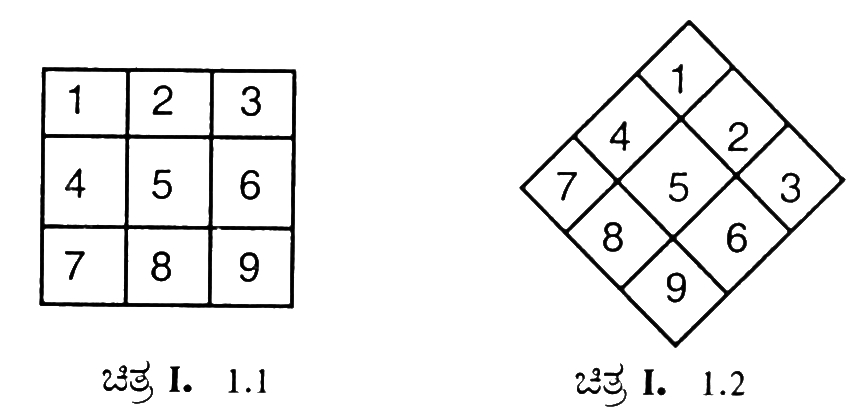
\includegraphics{src/figures/chap3/fig3-1.jpg}\\
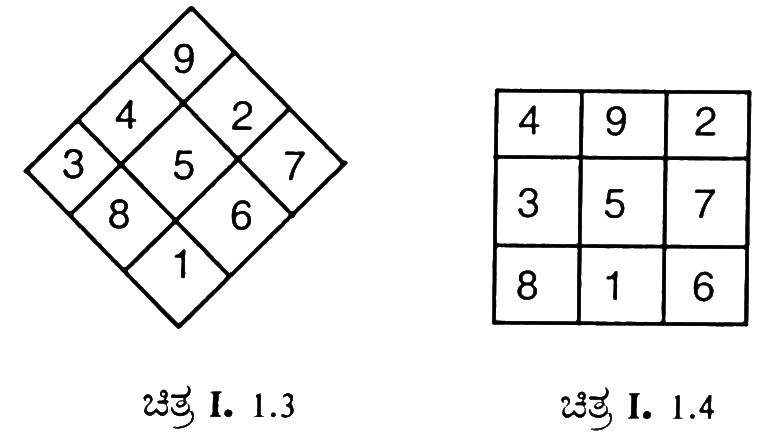
\includegraphics{src/figures/chap3/fig3-2.jpg}
\end{figure}

\begin{itemize}
	\item $3 \times 3$ ಚೌಕದಲ್ಲಿ 1ರಿಂದ 9ರವರೆಗಿನ ಅಂಕಿಗಳನ್ನು ಎಡ ಮೇಲ್ತುದಿಯ ಮನೆಯಿಂದ ಪ್ರಾರಂಭಿಸಿ, ಕ್ರಮವಾಗಿ ತುಂಬಿಸಿ. (ಚಿತ್ರ I.1.1)
	\item ಚೌಕವನ್ನು $45^\circ$ಗಳಷ್ಟು ಪ್ರದಕ್ಷಿಣವಾಗಿ ತಿರುಗಿಸಿ. (ಚಿತ್ರ I.1.2) ವಜ್ರಾಕೃತಿ ಲಭಿಸಿದೆ.
	\item ಶೃಂಗ ಮನೆಗಳಲ್ಲಿನ ಅಂಕಿಗಳನ್ನು ಎದುರು ಬದುರು ಮನೆಗಳಿಗೆ ಬದಲಾಯಿಸಿ (ಚಿತ್ರ I.1.3)
	\item ವಜ್ರಾಕೃತಿಯ ಮೇಲಿನ ತುದಿಯ (9) ಹಾಗೂ ಕೆಳಗಿನ ತುದಿಯ (1) ಮನೆಗಳ ಸಂಖ್ಯೆಗಳನ್ನು ಒಳಕ್ಕೆ ತಳ್ಳಿ.
	\item ಮತ್ತೆ ಚೌಕ ಲಭ್ಯ. (ಚಿತ್ರ II. 1.4) ಇದು ಮಾಯಾಚೌಕ. ಮೊತ್ತ 15.
	\item ಈ ವಿಧಾನ 3ನೆಯ ಕ್ರಮವರ್ಗಕ್ಕೆ ಮಾತ್ರ ಸುಲಭವಾಗಿ ಅನ್ವಯ.
\end{itemize}

\noindent \textbf{I (2) 3ನೆ ಕ್ರಮವರ್ಗದ ಮಾಯಾಚೌಕ ರಚನೆ : ವಿಧಾನ 2}

ಮಾಯಾಚೌಕದ ರಚನೆಯಲ್ಲಿ ತುಂಬಿಸಬೇಕಾದ ಸಂಖ್ಯೆಗಳು ಅಂಕಗಣಿತ ಶ್ರೇಢಿಯಲ್ಲಿ ರಬೇಕಾದುದು ಅಗತ್ಯ. ಉದಾಹರಣೆಗೆ 2,4,6,8,10........ಸಂಖ್ಯೆಗಳನ್ನು ಬಳಸಿ 3ನೇ ಕ್ರಮವರ್ಗದ ಒಂದು ಮಾಯಾಚೌಕ ರಚಿಸೋಣ.

\begin{itemize}
	\item $3 \times 3$ ರ ಒಂದು ಚೌಕ ರಚಿಸಿ. ಅದರ ಹೊರ ಸುತ್ತಿನ ಮಧ್ಯದ ನಾಲ್ಕು ಮನೆಗಳಿಗೂ ಅವುಗಳ ಹೊರ ಬದಿಗೆ ಒಂದೊಂದು ಮನೆ ರಚಿಸಿ ಚಿತ್ರ I. 2.1
	\begin{figure}[h]
	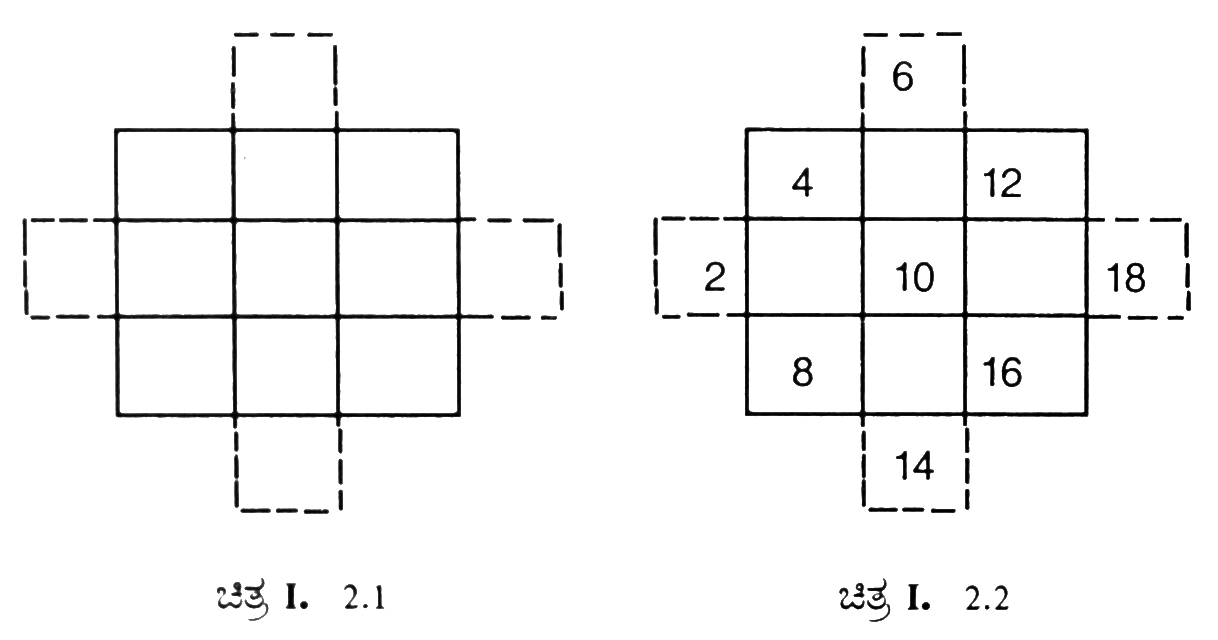
\includegraphics{src/figures/chap3/fig3-3.jpg}\\
	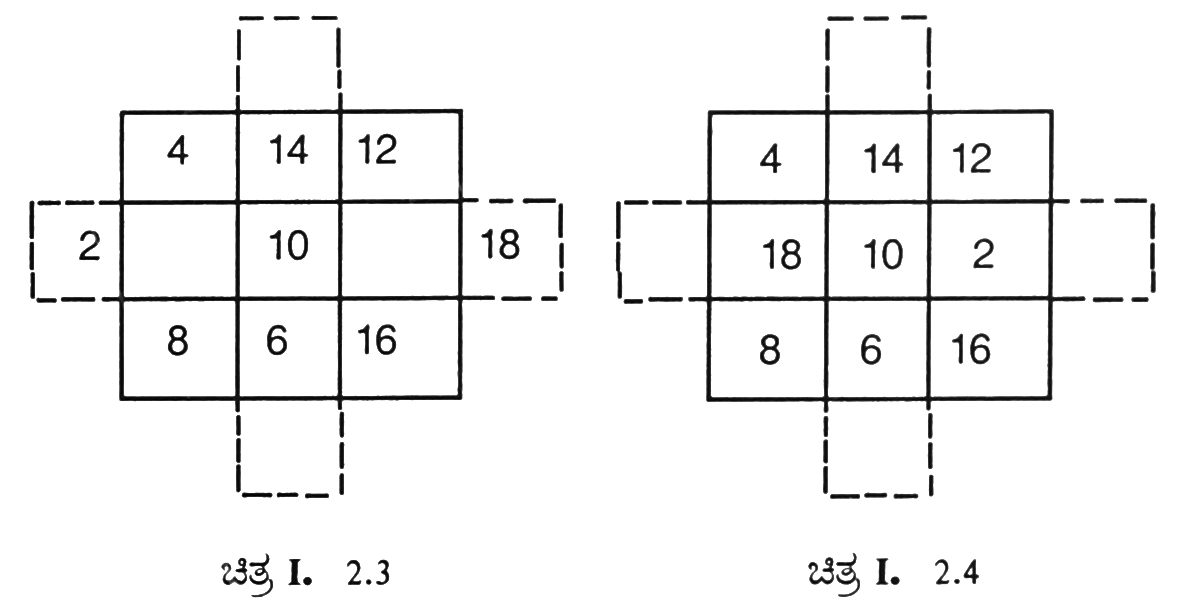
\includegraphics{src/figures/chap3/fig3-4.jpg}
	\end{figure}
	\item ಮಧ್ಯದ ಅಡ್ಡಸಾಲಿನ ಎಡಬದಿಯಲ್ಲಿ ರಚಿಸಿರುವ ಹೊಸ ಮನೆಯಿಂದ ಪ್ರಾರಂಭಿಸಿ, ಬಲಕ್ಕೆ ಓರೆಯಾಗಿ ಶ್ರೇಢಿಯ ಸಂಖ್ಯೆಗಳನ್ನು ಕ್ರಮವಾಗಿ ತುಂಬಿಸಿ. ಮೂಲ ಚೌಕದಲ್ಲಿಯೂ ಇದೇ ರೀತಿ ಮುಂದಿನ ಸಂಖ್ಯೆಗಳನ್ನು ತುಂಬಿಸಿ. ಕೆಳ ಬದಿಯಲ್ಲಿರುವ ಹೊಸ ಮನೆಯಿಂದ ಪ್ರಾರಂಭಿಸಿ ಕ್ರಮವಾಗಿ ಸಂಖ್ಯೆಗಳನ್ನು ತುಂಬಿಸಿ. ಚಿತ್ರ I. 2.2.
	\item ಹೊಸದಾಗಿ ರಚಿಸಿರುವ ಮನೆಗಳಲ್ಲಿನ ಸಂಖ್ಯೆಗಳನ್ನು ಅದೇ ಸಾಲಿನಲ್ಲಿ ಎದುರಿಗಿರುವ ಖಾಲಿ ಮನೆಯಲ್ಲಿ ತುಂಬಿಸಿ. ಚಿತ್ರ I. 2.3. ಮತ್ತು ಚಿತ್ರ I.2.4.
	\item ಮೊತ್ತ 30 ಇರುವ ಮಾಯಾಚೌಕ ಸಿದ್ಧ.
\end{itemize}

ಉದಾ: 5ನೇ ಕ್ರಮವರ್ಗ 1ರಿಂದ 25ರ ವರೆಗೆ ಸಂಖ್ಯೆಗಳು

ಇದೇ ವಿಧಾನವನ್ನನುಸರಿಸಿ 5,7,9..........ಕ್ರಮವರ್ಗದ ಮಾಯಾಚೌಕಗಳನ್ನು ರಚಿಸಬಹುದು. ಇವುಗಳ ಹೊರಸುತ್ತಿನಲ್ಲಿರುವ ಮನೆಗಳಲ್ಲಿ ಅಂಚಿನಲ್ಲಿರುವ ಮನೆಗಳನ್ನು ಹೊರತುಪಡಿಸಿ ಉಳಿದ ಮನೆಗಳ ಹೊರಬದಿಯಲ್ಲಿ ಮನೆಗಳನ್ನು ರಚಿಸಿ. 5ನೇ ಕ್ರಮವರ್ಗದ ಮಾಯಾಚೌಕವಾದರೆ, ಹೊಸದಾಗಿ ರಚಿಸಲ್ಪಟ್ಟ 3 ಮನೆಗಳ ಸಾಲು ನಾಲ್ಕು ಪಕ್ಕಗಳಲ್ಲಿರುತ್ತವೆ. ಹೊಸದಾಗಿ ರಚಿಸಿದ ಮೂರು ಮನೆಗಳ ಮಧ್ಯದ ಮನೆಯ ಹೊರಬದಿಗೆ ಒಂದೊಂದು ಮನೆ ರಚಿಸಿ.

ಶ್ರೇಢಿಯ ಸಂಖ್ಯೆಗಳನ್ನು ಮಧ್ಯದ ಅಡ್ಡಸಾಲಿನ ಎಡಪಕ್ಕದ ಮನೆಯಿಂದ ಪ್ರಾರಂಭಿಸಿ ಬಲಕ್ಕೆ ಓರೆಯಾಗಿ ತುಂಬಿಸಿ. ಕೆಳಬದಿಯ ಸಾಲುಗಳಲ್ಲೂ ಅದೇ ರೀತಿಯಲ್ಲಿ ಸಂಖ್ಯೆಗಳನ್ನು ತುಂಬಿಸಿ. ಚಿತ್ರ I. 2.5. ಹೊಸದಾಗಿ ರಚಿಸಿದ ಮನೆಗಳಲ್ಲಿರುವ ಸಂಖ್ಯೆಗಳನ್ನು ಅದೇ ಸಾಲಿನಲ್ಲಿ ಎದುರು ಬದಿಯಲ್ಲಿ ಮೂಲಚೌಕದ ಅತಿದೂರದಲ್ಲಿರುವ ಖಾಲಿ ಮನೆಯಲ್ಲಿ ತುಂಬಿಸಿ. ಚಿತ್ರ I. 2.6. ಮೊತ್ತ 65 ಇರುವ ಮಾಯಾಚೌಕ ಸಿದ್ಧ.
\begin{figure}[h]
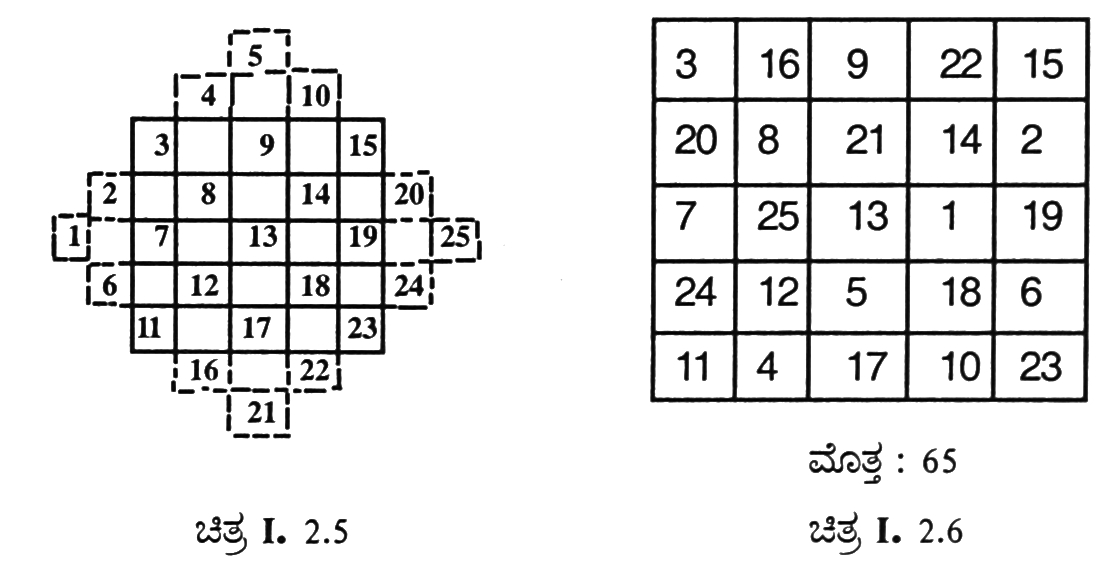
\includegraphics{src/figures/chap3/fig3-5.jpg}
\end{figure}

7ನೇ ಕ್ರಮವರ್ಗದ ಮಾಯಾಚೌಕ ರಚಿಸಬೇಕಾದಲ್ಲಿ, ಹೊರಬದಿಯಲ್ಲಿ 5,3,1 ಮನೆಗಳನ್ನು ನಾಲ್ಕೂ ಪಕ್ಷಗಳಲ್ಲಿ ರಚಿಸಿ, ಶ್ರೇಢಿಯ ಸಂಖ್ಯೆಗಳನ್ನು ತುಂಬಿಸಬೇಕು.

\noindent \textbf{I. 3. ಬೆಸಸಂಖ್ಯೆ  ಕ್ರಮವರ್ಗದ ಮಾಯಾಚೌಕ ರಚನೆಗೆ ಸಾಮಾನ್ಯ ವಿಧಾನ.}

ಈ ವಿಧಾನವನ್ನು ಯಾವುದೇ ಬೆಸಸಂಖ್ಯೆ ಕ್ರಮವರ್ಗದ ಮಾಯಾಚೌಕ ರಚನೆಗೂ ಬಳಸಬಹುದು. ತುಂಬಿಸಬೇಕಾದ ಸಂಖ್ಯೆಗಳು ಅಂಕಗಣಿತ ಶ್ರೇಢಿಯಲ್ಲಿರಬೇಕಾದುದು ಅಗತ್ಯ. ಒಂದು ಉದಾಹರಣೆಯಿಂದ ವಿಧಾನ ಸ್ಪಷ್ಟವಾಗಬಲ್ಲದು.

ಉದಾ : 3ನೇ ಕ್ರಮವರ್ಗ ; 1ರಿಂದ 9ರ ವರೆಗಿನ ಕ್ರಮಾಗತ ಸಂಖ್ಯೆಗಳು.
\begin{itemize}
	\item $3 \times 3$ ರ ಚೌಕ ರಚಿಸಿ
	\item ಮೇಲಿನ ಅಡ್ಡಸಾಲಿನ ಮಧ್ಯದ ಮನೆಯಲ್ಲಿ 1 ಬರೆಯಿರಿ. ಚಿತ್ರ I. 3.1
	\item ಬಲಗಡೆಗೆ ಓರೆಯಾಗಿ ಮೇಲಕ್ಕೆ ಚಲಿಸಿ. ಚಿತ್ರ I. 3.1 ರಲ್ಲಿ ಬಾಣದ ಗುರುತು ಗಮನಿಸಿ.
	\item ಮನೆ ಇಲ್ಲ. ಅದೇ ಸಾಲಿನ ಕೊನೆ ಮನೆಗೆ ಮುಂದಿನ ಸಂಖ್ಯೆ ತುಂಬಿಸಿ. ಚಿತ್ರ I.3.2.
	\item ಬಲಕ್ಕೆ ಓರೆಯಾಗಿ ಚಲಿಸಿ. ಮನೆ ಇಲ್ಲ. ಅದೇ ಸಾಲಿನ ಕೊನೇ ಮನೆಗೆ ಮುಂದಿನ ಸಂಖ್ಯೆ ತುಂಬಿಸಿ. ಚಿತ್ರ I. 3.3.
	\item ಮತ್ತೆ ಬಲಕ್ಕೆ ಓರೆಯಾಗಿ ಚಲಿಸಿ. ಮನೆ ತುಂಬಿದೆ. ಆದ್ದರಿಂದ ಒಂದು ಮನೆ ಕೆಳಕ್ಕೆ ಚಲಿಸಿ. ಚಿತ್ರ I. 3.4. ಓರೆಯಾಗಿ ಕೊನೆಯ ಮನೆವರೆಗೆ ಮುಂದಿನ ಸಂಖ್ಯೆಗಳನ್ನು ತುಂಬಿಸಿ.
	\item ಬಲಕ್ಕೆ ಓರೆಯಾಗಿ ಚಲಿಸಿ. ಮನೆ ಇಲ್ಲ. ಅದೇ ಸಾಲಿನ ಕೆಳಗಿನ ಮನೆಗೆ ಮುಂದಿನ ಸಂಖ್ಯೆ ತುಂಬಿಸಿ. ಚಿತ್ರ I. 3.5.
	\item ಬಲಕ್ಕೆ ಓರೆಯಾಗಿ ಚಲಿಸಿ. ಮನೆ ಇಲ್ಲ. ಅದೇ ಸಾಲಿನ ಕೊನೆಯ ಮನೆಗೆ ಮುಂದಿನ ಸಂಖ್ಯೆ ತುಂಬಿಸಿ. ಚಿತ್ರ I. 3.6.
	\item ಬಲಕ್ಕೆ ಓರೆಯಾಗಿ ಚಲಿಸಿ. ಮನೆ ಇಲ್ಲ. ಅದೇ ಕಂಭಸಾಲಿನ ಕೊನೆಯ ಮನೆಗೆ ಮುಂದಿನ ಸಂಖ್ಯೆ ತುಂಬಿಸಿ. ಚಿತ್ರ I. 3.7
	\item ಮಾಯಾ ಚೌಕ ಸಿದ್ಧ. ಮೊತ್ತ 15 ಚಿತ್ರ I. 3.8
	\begin{figure}[h]
	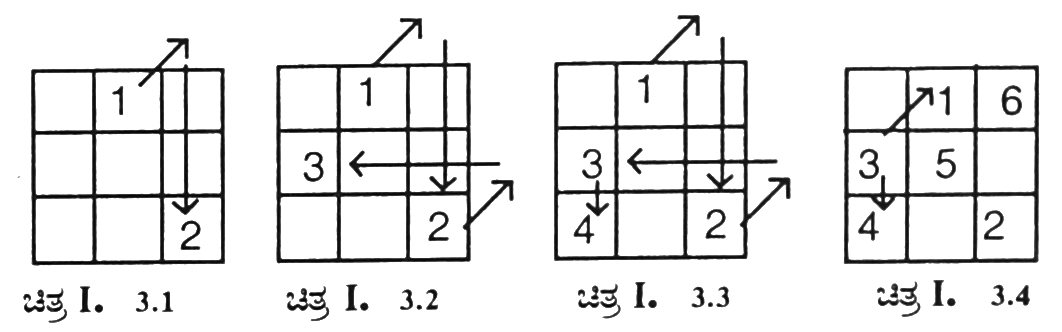
\includegraphics{src/figures/chap3/fig3-6.jpg}\\
	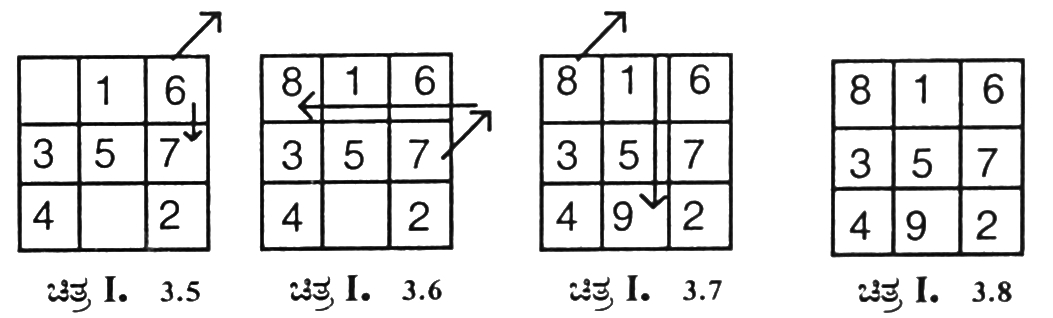
\includegraphics{src/figures/chap3/fig3-7.jpg}
	\end{figure}
	ಈ ಮೇಲಿನ ವಿಧಾನದಿಂದ ರಚಿಸಿರುವ 5ನೇ ಮತ್ತು 7ನೇ ಕ್ರಮವರ್ಗಗಳ ಮಾಯಾಚೌಕಗಳನ್ನು ಅವಗಾಹನೆಗಾಗಿ ಕೊಟ್ಟಿದೆ.
	\begin{figure}[h]
	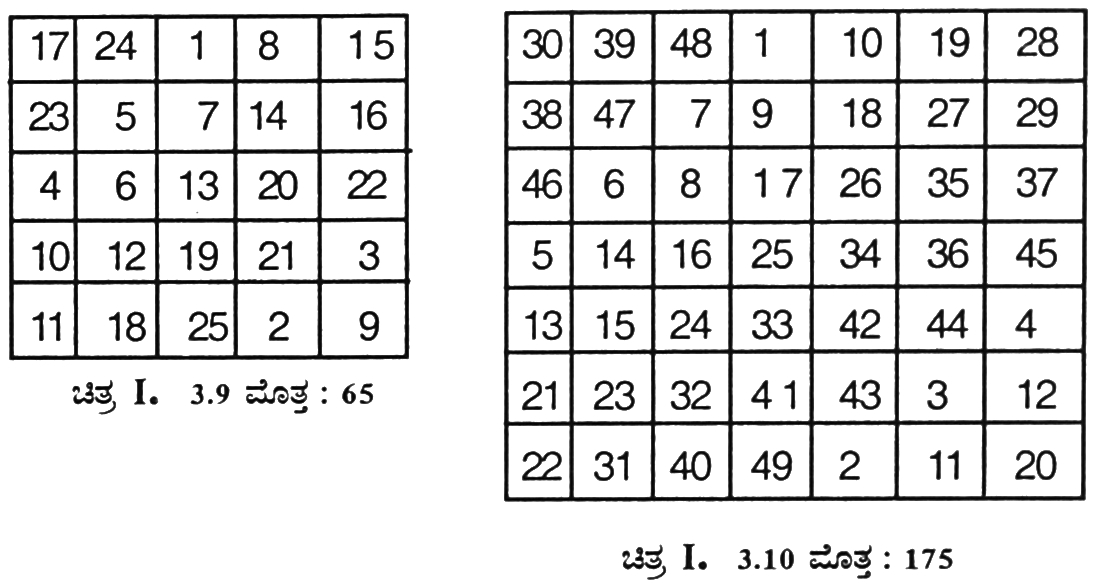
\includegraphics{src/figures/chap3/fig3-8.jpg}
	\end{figure}
\end{itemize}

\noindent \textbf{ಈ ವಿಧಾನದಲ್ಲಿ ಮಾಯಾಚೌಕ ರಚಿಸಲು ನೆನಪಿನಲ್ಲಿರಬೇಕಾದ ಅಂಶಗಳು :}
\begin{itemize}
	\item ತುಂಬಿಸಬೇಕಾದ ಸಂಖ್ಯೆಗಳು ಅಂಕಗಣಿತ ಶ್ರೇಢಿಯಲ್ಲಿರುವುದು ಅಗತ್ಯ. ಶ್ರೇಢಿಯ ಮೊದಲ ಸಂಖ್ಯೆಯನ್ನು ಚೌಕದ ಮೇಲಿನ ಅಡ್ಡಸಾಲಿನ ಮಧ್ಯದ ಮನೆಯಲ್ಲಿ ತುಂಬಿಸಬೇಕು.
	\item ಬಲಕ್ಕೆ ಓರೆಯಾಗಿ ಚಲಿಸಬೇಕು.
	\item ಕಂಭಸಾಲಿನ ಮೇಲಕ್ಕೆ ಅಥವಾ ಅಡ್ಡಸಾಲಿನ ಬಲಕ್ಕೆ ಬಂದಾಗ ಆ ಸಾಲಿನ ಕೊನೆಯ ಖಾಲಿ ಮನೆ ತುಂಬಿಸಬೇಕು.
	\item ತುಂಬಿದ ಮನೆ ಎದುರಾದರೆ ಅಥವಾ ಯಾವುದೇ ಸಾಲುಗಳು ಇಲ್ಲದಾಗ (3.9ರಲ್ಲಿ 15, 3.10ರಲ್ಲಿ 28, 3.5ರಲ್ಲಿ 6) ಕೆಳಗಿನ ಮನೆ ತುಂಬಿಸಬೇಕು.
	\item ಈ ವಿಧಾನಕ್ಕೆ ಡಿ.ಲಾ ಲೂಬೆರೆ (De La Loubere) ವಿಧಾನವೆಂದು ಹೆಸರಿದೆ. 1693ರಲ್ಲಿ ಸೈಮನ್ ಡಿ.ಲಾ ಲೂಬೆರೆಯು ಇದನ್ನು ಪ್ರಸ್ತುತ ಪಡಿಸಿದ. 14ನೇ ಲೂಯಿಯ ಆಸ್ಥಾನದಿಂದ ಸಯಾಂನಲ್ಲಿ ರಾಯಭಾರಿಯಾಗಿದ್ದಾಗ ಆತ ಸಯಾಂನಲ್ಲಿ ಈ ವಿಧಾನ ಕಲಿತೆನೆಂದು ಹೇಳಿದ್ದಾನೆ.
\end{itemize}

\noindent \textbf{I. 4.ಬೆಸಸಂಖ್ಯೆ ಕ್ರಮವರ್ಗದ ಮಾಯಾಚೌಕ ರಚಿಸಲು ಅನೇಕವಿಧಾನಗಳಿವೆ.}

ಈಗ ಮತ್ತೊಂದು ವಿಧಾನವನ್ನು ಪರಿಶೀಲಿಸೋಣ.

ಉದಾಹರಣೆಗೆ : 3ನೇ ಕ್ರಮವರ್ಗದ ಒಂದು ಮಾಯಾಚೌಕ ರಚಿಸೋಣ. ಅಂಕಗಣಿತ ಶ್ರೇಢಿಯಲ್ಲಿರುವ ಮೂರು ಸಂಖ್ಯೆಗಳ ಎರಡು ಗುಂಪುಗಳನ್ನು ತೆಗೆದುಕೊಳ್ಳಿ.

ಅವು 1,2, 3 ಮತ್ತು 7, 11, 15 ಇರಲಿ.
\begin{figure}[h]
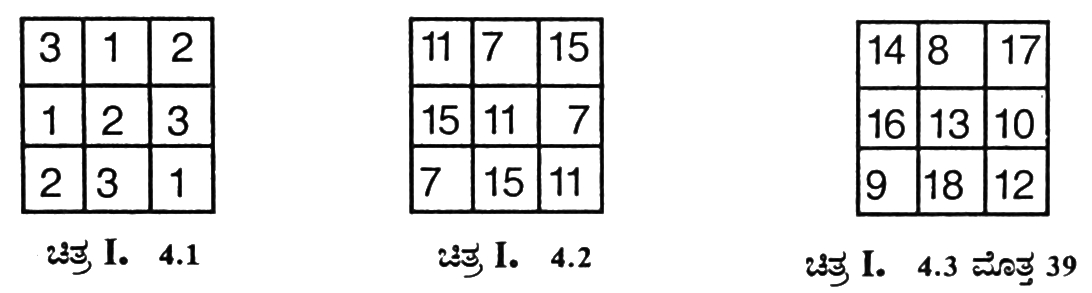
\includegraphics{src/figures/chap3/fig3-9.jpg}
\end{figure}

\begin{itemize}
	\item $3 \times 3$ ಮೂರು ಚೌಕಗಳನ್ನು ರಚಿಸಿ.
	\item ಮೊದಲ ಚೌಕದ (I.4.1) ಮೊದಲ ಅಡ್ಡಸಾಲಿನಲ್ಲಿ ಒಂದು ಅಂಕಗಣಿತ ಶ್ರೇಢಿಯ ಮೂರು ಸಂಖ್ಯೆಗಳನ್ನು ಯಾವುದೇ ಕ್ರಮದಲ್ಲಿ ತುಂಬಿಸಿ.
	\item ಅದೇ ಚೌಕದ ಎರಡನೆ ಅಡ್ಡಸಾಲಿನಲ್ಲಿ ಮೊದಲ ಅಡ್ಡಸಾಲಿನ ಮಧ್ಯದ ಮನೆಯ ಸಂಖ್ಯೆಯಿಂದ (ಇಲ್ಲಿ 1) ಪ್ರಾರಂಭಿಸಿ, ಕ್ರಮವಾಗಿ ಸಂಖ್ಯೆಗಳನ್ನು ತುಂಬಿಸಿ. (1,2) ಕೊನೆಯ ಮನೆಯಲ್ಲಿ ಮೊದಲ ಅಡ್ಡಸಾಲಿನ ಮೊದಲ ಮನೆಯ ಸಂಖ್ಯೆ ತುಂಬಿಸಿ. (1,2,3)
	\item ಮೂರನೆಯ ಅಡ್ಡಸಾಲಿನ ಮೊದಲ ಮನೆಯಲ್ಲಿ ಎರಡನೆ ಅಡ್ಡಸಾಲಿನ ಮಧ್ಯದ ಮನೆಯ ಸಂಖ್ಯೆಯಿಂದ (2) ಪ್ರಾರಂಭಿಸಿ, ಕ್ರಮವಾಗಿ ಸಂಖ್ಯೆಗಳನ್ನು ತುಂಬಿಸಿ, (2,3) ಕೊನೆಯ ಮನೆಯನ್ನು ಎರಡನೆ ಅಡ್ಡಸಾಲಿನ ಮೊದಲ ಸಂಖ್ಯೆಯಿಂದ ತುಂಬಿಸಿ. (2,3,1) ಚಿತ್ರ I.4.1. ನೋಡಿ
	\item ಎರಡನೆ ಚೌಕ (I.4.2) ಮೊದಲ ಅಡ್ಡಸಾಲಿನಲ್ಲಿ ಇನ್ನೊಂದು ಗುಂಪಿನ ಮೂರು ಸಂಖ್ಯೆಗಳನ್ನು ಯಾವುದೇ ಕ್ರಮದಲ್ಲಿ ತುಂಬಿಸಿ.
	\item ಇದೇ ಚೌಕದ ಎರಡನೆ ಅಡ್ಡಸಾಲಿನ ಮೊದಲ ಮನೆಯನ್ನು ಮೊದಲ ಅಡ್ಡಸಾಲಿನ ಕೊನೆಯ ಮನೆಯಲ್ಲಿನ ಸಂಖ್ಯೆಯಿಂದ (15) ತುಂಬಿಸಿ. ಉಳಿದ ಮನೆಗಳನ್ನು ಕ್ರಮವಾಗಿ ಉಳಿದ ಸಂಖ್ಯೆಗಳಿಂದ (11,7) ತುಂಬಿಸಿ. (ಚಿತ್ರ I.4.2) ನೋಡಿ
	\item I.4.3 ಚೌಕದಲ್ಲಿ ಮೊದಲೆರಡು ಚೌಕಗಳ ಅನುರೂಪ ಮನೆಗಳಲ್ಲಿನ ಸಂಖ್ಯೆಗಳ ಮೊತ್ತವನ್ನು ಬರೆಯಿರಿ. 3+11=14 ಮೊದಲ ಮನೆ ಇತ್ಯಾದಿ.

	I.4.3 ಮಾಯಾಚೌಕ. ಮೊತ್ತ 39.

	ಇದೇ ವಿಧಾನದಿಂದ ರಚಿಸಿರುವ ಮತ್ತೊಂದು ಉದಾಹರಣೆ.
	\begin{figure}[h]
	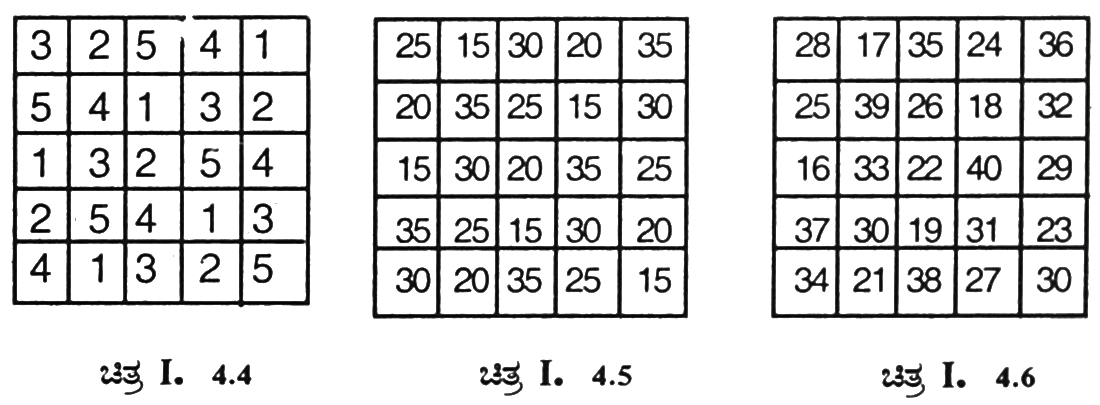
\includegraphics{src/figures/chap3/fig3-10.jpg}
	\end{figure}

	\textbf{ಗಮನಿಸಿ :}
	\item ತೆಗೆದುಕೊಂಡಿರುವ ಅಂಕಗಣಿತ ಶ್ರೇಢಿಗಳು 1,2, 3,4, 5 ಮತ್ತು 15,20,25,30,35
	\item ಮೊದಲ ಅಡ್ಡಸಾಲುಗಳಲ್ಲಿ ಶ್ರೇಢಿಯ ಸಂಖ್ಯೆಗಳನ್ನು ಯಾದೃಚ್ಛಿಕವಾಗಿ (Random) ತುಂಬಿಸಿದೆ.
	\item I.4.4ರಲ್ಲಿ ಎರಡನೆ ಅಡ್ಡಸಾಲನ್ನು ಮೊದಲ ಅಡ್ಡಸಾಲಿನ ಮಧ್ಯದ ಮನೆಯ ಸಂಖ್ಯೆಯಿಂದ ಪ್ರಾರಂಭಿಸಿ ಕ್ರಮವಾಗಿ ತುಂಬಿಸಿದೆ. ಉಳಿದ ಅಡ್ಡಸಾಲುಗಳಲ್ಲೂ ಇದೇ ಕ್ರಮವನ್ನು ಅನುಸರಿಸಿದೆ.
	\item I.4.5ರಲ್ಲಿ ಎರಡನೆ ಅಡ್ಡಸಾಲನ್ನು ಮೊದಲ ಅಡ್ಡಸಾಲಿನ ಕೊನೆಯ ಎರಡು ಸಂಖ್ಯೆಗಳಿಂದ ಮೊದಲು ಮಾಡಿ ಕ್ರಮವಾಗಿ ತುಂಬಿಸಿದೆ. ಉಳಿದ ಅಡ್ಡಸಾಲುಗಳಲ್ಲೂ ಇದೇ ಕ್ರಮ ಅನುಸರಿಸಿದೆ.
	\item I.4.6ರಲ್ಲಿ ಉಳಿದ ಎರಡು ಚೌಕಗಳ ಅನುರೂಪ ಮನೆಗಳಲ್ಲಿನ ಸಂಖ್ಯೆಗಳ ಮೊತ್ತದಿಂದ ತುಂಬಿಸಿದೆ. ಇದು ಮಾಯಾಚೌಕ.

	ಮೊತ್ತ : 140
\end{itemize}
ಇದೇ ವಿಧಾನವನ್ನು ಬಳಸಿ.7,9,........ಕ್ರಮವರ್ಗ (Order) ಮಾಯಾ ಚೌಕಗಳನ್ನು ರಚಿಸಬಹುದು. ಕೆಲವು ವೇಳೆ ಮಾಯಾಚೌಕದಲ್ಲಿ ಸಂಖ್ಯೆಗಳು ಪುನರಾವರ್ತಿತವಾಗಬಹುದು. ಶ್ರೇಢಿಗಳನ್ನು ಸೂಕ್ತವಾಗಿ ಬದಲಾಯಿಸಿ ಪುನರಾವರ್ತನೆಯನ್ನು ನಿವಾರಿಸಬಹುದು.

\section*{I. 5 ಪೂರಕ ಚೌಕ ವಿಧಾನ}

ಈ ಹಿಂದೆ ಹೇಳಿದ ವಿಧಾನದಲ್ಲಿ (I.4) ತೆಗೆದುಕೊಳ್ಳುವ ಸಂಖ್ಯಾ ಗುಂಪುಗಳೆರಡೂ ಅಂಕಗಣಿತ ಶ್ರೇಢಿಯಲ್ಲಿರಬೇಕೆಂದು ಹೇಳಿತ್ತಲ್ಲವೇ? ಪೂರಕ ಚೌಕ ವಿಧಾನದಲ್ಲಿ ಒಂದು ಗುಂಪು ಮಾತ್ರ ಅಂಕಗಣಿತ ಶ್ರೇಢಿಯಲ್ಲಿದ್ದರೆ ಸಾಕು. ಇನ್ನೊಂದು ಗುಂಪು ಯಾವುದೇ ಸಂಖ್ಯೆಗಳನ್ನು ಹೊಂದಿರಬಹುದು. ಪ್ರತಿಗುಂಪಿನಲ್ಲಿಯೂ ಅಪೇಕ್ಷಿತ ಮಾಯಾಚೌಕವು ಎಷ್ಟನೆಯ ಕ್ರಮವರ್ಗದ್ದೋ (Order) ಅಷ್ಟು ಸಂಖ್ಯೆಗಳಿರಬೇಕು. ನೆನಪಿಡಿ. ಈ ವಿಧಾನವು ಬೆಸಸಂಖ್ಯೆ ಕ್ರಮವರ್ಗದ ಮಾಯಾಚೌಕ ರಚನೆಗೆ ಮಾತ್ರ.

\textbf{ಈ ವಿಧಾನದಲ್ಲಿ 3 ಹಂತಗಳಿವೆ.}

\textbf{(ಅ) ಮೂಲ ಚೌಕ ರಚನೆ}

\textbf{(ಬ) ಪೂರಕ ಚೌಕ ರಚನೆ}

\textbf{(ಕ) ಮಾಯಾ ಚೌಕ ರಚನೆ}

ಒಂದು ಉದಾಹರಣೆ ನೋಡೋಣ. ಅಪೇಕ್ಷಿತ ಮಾಯಾಚೌಕವು 5ನೇ ಕ್ರಮವರ್ಗದ್ದು ಆಗಿರಲಿ.

\subsection*{ಮೂಲ ಚೌಕ ರಚನೆ :}

ಯಾವುದೇ 5 ಸಂಖ್ಯೆಗಳನ್ನು ತೆಗೆದುಕೊಳ್ಳಿ. ಅವು ಅಂಕಗಣಿತಶ್ರೇಢಿಯಲ್ಲಿರಬೇಕಾದ ಅಗತ್ಯವಿಲ್ಲ. ಅವು 3,7,9,11,15 ಇರಲಿ.
\begin{itemize}
	\item $5 \times 5$ರ ಒಂದು ಚೌಕ ರಚಿಸಿ.
	\item ಮೊದಲ ಅಡ್ಡಸಾಲಿನಲ್ಲಿ 5 ಸಂಖ್ಯೆಗಳನ್ನು ಯಾವ ಕ್ರಮದಲ್ಲಿಯಾದರೂ ಬರೆಯಿರಿ. ಚಿತ್ರ.I.5.1.ನೋಡಿ
	\item ಮೊದಲ ಅಡ್ಡಸಾಲಿನ ಕೊನೆಯ ಎರಡು ಸಂಖ್ಯೆಗಳಿಂದ ಮೊದಲು ಮಾಡಿ ಎರಡನೆಯ ಅಡ್ಡಸಾಲನ್ನು ತುಂಬಿಸಿ. ಆ ಸಾಲಿನಲ್ಲಿ ಉಳಿದ ಮೂರು ಮನೆಗಳನ್ನು ಮೊದಲ ಅಡ್ಡಸಾಲಿನ ಉಳಿದ ಮೂರು ಸಂಖ್ಯೆಗಳಿಂದ ಅದೇ ಕ್ರಮದಲ್ಲಿ ತುಂಬಿಸಿ. ಚಿತ್ರ.I. 5.2.ನೋಡಿ.
	\item 3,4 ಮತ್ತು 5ನೆಯ ಅಡ್ಡಸಾಲುಗಳನ್ನು ಇದೇ ರೀತಿ ಅಂದರೆ ಹಿಂದಿನ ಸಾಲಿನ ಕೊನೆಯ 2 ಸಂಖ್ಯೆಗಳಿಂದ ಪ್ರಾರಂಭಿಸಿ, ನಂತರ ಮೊದಲ 3 ಸಂಖ್ಯೆಗಳನ್ನು ಆ ಸಾಲಿನ ಕೊನೆಯ ಮೂರು ಮನೆಗಳಲ್ಲಿ ತುಂಬಿಸುವುದು. ಇದು ಮೂಲ ಚೌಕ ಚಿತ್ರ.I.5.3.

	\begin{figure}[h]
	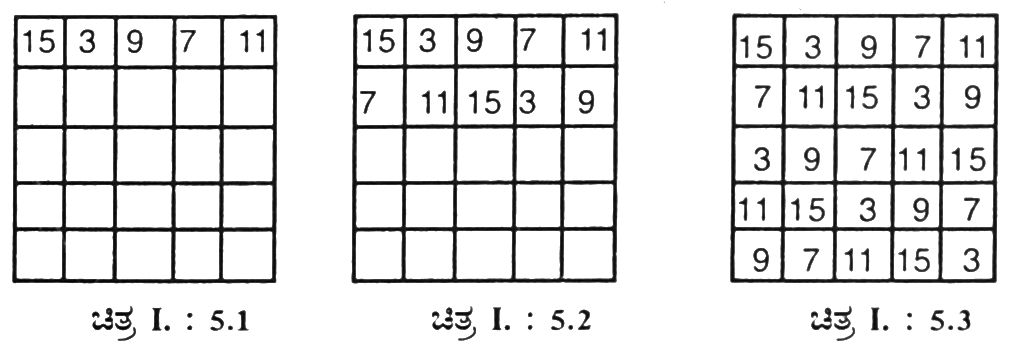
\includegraphics{src/figures/chap3/fig3-11.jpg}
	\end{figure}
\end{itemize}

\subsection*{ಪೂರಕ ಚೌಕ ರಚನೆ :}

\begin{itemize}
	\item ಅಂಕಗಣಿತ ಶ್ರೇಢಿಯಲ್ಲಿರುವ ಯಾವುದಾದರೂ 5 ಸಂಖ್ಯೆಗಳನ್ನು ತೆಗೆದುಕೊಳ್ಳಿ.

	ಉದಾ : 0,5,10,15,20
	\item ಈ ಸಂಖ್ಯೆಗಳನ್ನು ಒಂದು $5 \times 5$ ಚೌಕದ ಮೊದಲ ಅಡ್ಡಸಾಲಿನಲ್ಲಿ ಯಾವುದೇ ಕ್ರಮದಲ್ಲಿ ತುಂಬಿಸಿ. ಚಿತ್ರ. I. 5.4
	\item ಮೊದಲ ಅಡ್ಡಸಾಲಿನ ಕೊನೆಯ ಮೂರು ಸಂಖ್ಯೆಗಳಿಂದ ಮೊದಲು ಮಾಡಿ ಎರಡನೆ ಅಡ್ಡಸಾಲು ತುಂಬಿಸಿ. ಮೂರು ಸಂಖ್ಯೆಗಳ ನಂತರ ಮೊದಲ ಎರಡು ಸಂಖ್ಯೆಗಳನ್ನು ಕ್ರಮವಾಗಿ ತುಂಬಿಸಿ. ಇದೇ ರೀತಿ 3, 4 ಮತ್ತು 5ನೆಯ ಅಡ್ಡಸಾಲುಗಳನ್ನು ತುಂಬಿಸಿ. ಪ್ರತಿ ಅಡ್ಡಸಾಲಿನಲ್ಲಿಯೂ ಅದರ ಹಿಂದಿನ ಅಡ್ಡಸಾಲಿನ ಕೊನೆಯ ಮೂರು ಸಂಖ್ಯೆಗಳು ಮೊದಲು ಬಂದು, ಕೊನೆಯ ಎರಡು ಸಂಖ್ಯೆಗಳು ಅಂತ್ಯದಲ್ಲಿರುತ್ತವೆ. ಈಗ ಪೂರಕ ಚೌಕ ಸಿದ್ಧ. ಚಿತ್ರ. I.5.5.
	\begin{figure}[h]
	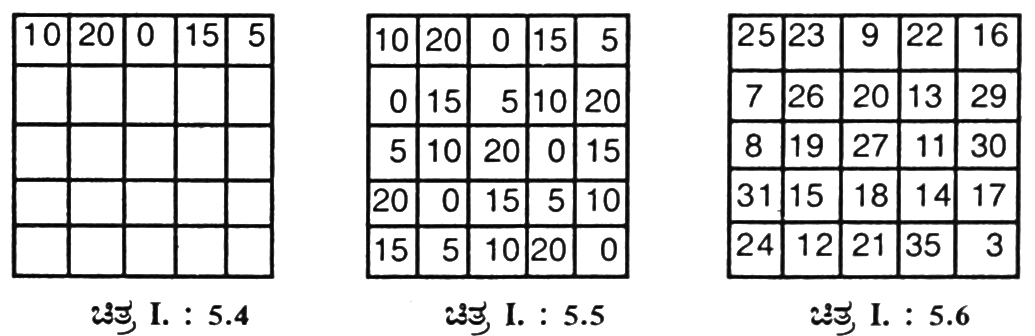
\includegraphics{src/figures/chap3/fig3-12.jpg}
	\end{figure}
\end{itemize}
\subsection*{ಮಾಯಾಚೌಕ ರಚನೆ :}

\begin{itemize}
	\item ಇನ್ನೊಂದು $5 \times 5$ ಚೌಕ ರಚಿಸಿ.
	\item ಮೂಲ ಚೌಕ ಮತ್ತು ಪೂರಕ ಚೌಕಗಳಲ್ಲಿನ ಅನುರೂಪ ಮನೆಗಳಲ್ಲಿರುವ ಸಂಖ್ಯೆಗಳನ್ನು ಕೂಡಿಸಿ ಈ ಚೌಕದಲ್ಲಿ ಬರೆಯಿರಿ. ಚಿತ್ರ. I. 5.6
	ಉದಾ: 15+10=25 ಮೊದಲ ಮನೆಯಲ್ಲಿ .

	ಮಾಯಾಚೌಕ ಲಭ್ಯ. ಮೊತ್ತ 95

	ಈ ವಿಧಾನದಲ್ಲಿ 3,7,9.......ಬೆಸಸಂಖ್ಯೆ ಕ್ರಮವರ್ಗದ ಮಾಯಾಚೌಕಗಳನ್ನು ರಚಿಸಬಹುದು. ಸಮಸಂಖ್ಯೆ ಕ್ರಮವರ್ಗಗಳ ಮಾಯಾಚೌಕ ರಚಿಸಲು ಈ ವಿಧಾನದಂತೆ ಸಾಧ್ಯವಿಲ್ಲ.
\end{itemize}

ಅಪೇಕ್ಷಿತ ಮೊತ್ತ ಬರುವಂತೆ ಮಾಯಾಚೌಕ ರಚಿಸಬಹುದು. ಇಂತಹ ಸಂದರ್ಭದಲ್ಲಿ ಮೂಲ ಚೌಕ, ಪೂರಕ ಚೌಕ ರಚಿಸಲು ತೆಗೆದುಕೊಳ್ಳುವ ಸಂಖ್ಯೆಗಳ ಮೊತ್ತ ಅಪೇಕ್ಷಿತ ಮೊತ್ತಕ್ಕೆ ಸಮವಾಗಿರಬೇಕು. ಕೆಲವೊಮ್ಮೆ ಅಂತಿಮ ಮಾಯಾಚೌಕದಲ್ಲಿ ಸಂಖ್ಯೆಗಳು ಪುನರಾವರ್ತಿತ ವಾಗಬಹುದು. ಮೂಲಚೌಕದ ಸಂಖ್ಯೆಗಳ ಮೊತ್ತ ವ್ಯತ್ಯಾಸವಾಗದಂತೆ, ಅವುಗಳನ್ನು ಬದಲಾಯಿಸಿ ಪುನರಾವರ್ತನೆಯನ್ನು ನಿವಾರಿಸಬಹುದು.

ಉದಾಹರಣೆಗೆ : 100 ಮೊತ್ತ ಬರುವಂತೆ ಒಂದು 5ನೇ ಕ್ರಮವರ್ಗದ ಮಾಯಾಚೌಕವನ್ನು ಪೂರಕ ಚೌಕ ವಿಧಾನದಿಂದ ರಚಿಸೋಣ.

ಒಂದು ಅಂಕಗಣಿತ ಶ್ರೇಢಿ 0,3,6,9,12ಇರಲಿ. ಮೊತ್ತ 30.

ಇನ್ನೊಂದು 5 ಸಂಖ್ಯೆಗಳ ಗುಂಪು, ಅವುಗಳ ಮೊತ್ತ 70 ಆಗುವಂತೆ ಆಯ್ಕೆ ಮಾಡಿ.

2,6,13,22,27 ಇರಲಿ. ಮೊತ್ತ 70 ಆಗುತ್ತದೆ.

\begin{itemize}
	\item $5 \times 5$ರ ಮೂರು ಚೌಕ ರಚಿಸಿ. ಚಿತ್ರ. I.5.7, I.5.8 ಮತ್ತು I.5.9
	\item ಚಿತ್ರ. I.5.7,ಚೌಕದಲ್ಲಿ 2,6,13,22,27 ಇವುಗಳನ್ನು ಮೊದಲ ಅಡ್ಡಸಾಲಿನಲ್ಲಿ ಯಾವುದೇ ಕ್ರಮದಲ್ಲಿ ಬರೆಯಿರಿ.
	\item ಕೊನೆಯ 2ಸಂಖ್ಯೆಗಳಿಂದ ಮುಂದಿನ ಅಡ್ಡಸಾಲನ್ನು ಶುರುಮಾಡಿ. ತುಂಬಿಸಿ.
	\item ಇದೇ ರೀತಿ ಉಳಿದ ಅಡ್ಡಸಾಲುಗಳನ್ನೂ ತುಂಬಿಸಿ. ಚಿತ್ರ. I.5.7ನೋಡಿ.
	\item ಚಿತ್ರ. I.5.8 ಚೌಕದ ಮೊದಲ ಅಡ್ಡಸಾಲಿನಲ್ಲಿ ಅಂಕಗಣಿತ ಶ್ರೇಢಿಯಲ್ಲಿರುವ ಸಂಖ್ಯೆಗಳನ್ನು ಯಾವುದೇ ಕ್ರಮದಲ್ಲಿ ತುಂಬಿಸಿ.
	\item ಕೊನೆಯ 3 ಸಂಖ್ಯೆಗಳಿಂದ ಪ್ರಾರಂಭಿಸಿ ಎರಡನೆ ಅಡ್ಡಸಾಲನ್ನು ತುಂಬಿಸಿ.
	\item ಇದೇ ರೀತಿ ಉಳಿದ ಅಡ್ಡಸಾಲುಗಳನ್ನು ತುಂಬಿಸಿ. ಚಿತ್ರ. I.5.8. ನೋಡಿ
	\item ಚಿತ್ರ. I.5.9 ಚೌಕದಲ್ಲಿನ ಮನೆಗಳನ್ನು ಮೊದಲೆರಡು ಚೌಕಗಳ ಅನುರೂಪ (Corresponding) ಮನೆಗಳಲ್ಲಿನ ಸಂಖ್ಯೆಗಳ ಮೊತ್ತದಿಂದ ತುಂಬಿಸಿ. ಲಭಿಸುವುದು 5ನೇ ಕ್ರಮವರ್ಗ (Order) ಮಾಯಾಚೌಕ. ಮೊತ್ತ 100.

	\begin{figure}[h]
	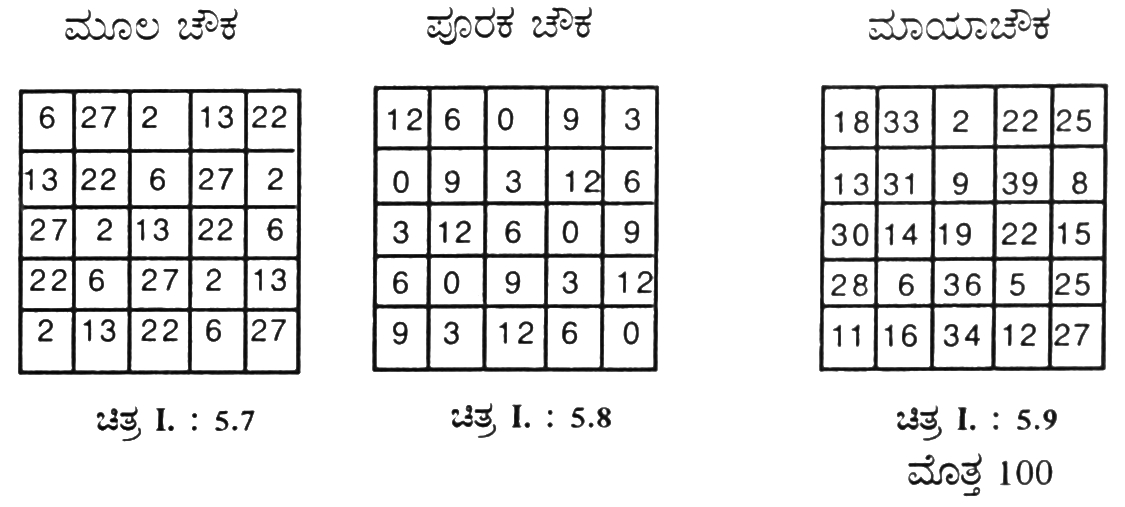
\includegraphics{src/figures/chap3/fig3-13.jpg}
	\end{figure}
\end{itemize}

\section*{II. ಸಮಸಂಖ್ಯೆ ಕ್ರಮವರ್ಗದ ಮಾಯಾಚೌಕ ರಚನೆ :}

2,4,6,8,10,12,14......ಇವುಗಳು ಸಮಸಂಖ್ಯೆಗಳು. ಇವುಗಳನ್ನು ಎರಡು ಗುಂಪುಗಳಾಗಿ ವಿಂಗಡಿಸಬಹುದು.

\begin{itemize}
	\item $2 (2n+1)$ ರೂಪದವು.

	$n=1$ ಆದಾಗ 6

	$n=2$ ಆದಾಗ 10

	$n=3$ ಆದಾಗ 14

	.........................ಇತ್ಯಾದಿ

	6,10,14,18,22,26........................................................ಇತ್ಯಾದಿ
	\item $4n$ ರೂಪದವು. 

	$n=1$ ಆದಾಗ 4

	$n=2$ ಆದಾಗ 8

	$n=3$ ಆದಾಗ 12

	.........................ಇತ್ಯಾದಿ

	4,8,12,16,20,24................................ಇತ್ಯಾದಿ

	\{ 2 ಸಮಸಂಖ್ಯೆ. 2 ಕ್ರಮವರ್ಗದ ಮಾಯಾಚೌಕದಲ್ಲಿ ನಾಲ್ಕು ಮನೆಗಳಲ್ಲಿಯೂ ಒಂದೇ ಸಂಖ್ಯೆ ಇರಬೇಕಾಗುತ್ತದೆ. ಹಾಗಾಗಿ ಇದನ್ನು ಪರಿಗಣಿಸುವುದಿಲ್ಲ \}

	ಮೇಲಿನ ಎರಡೂ ಗುಂಪುಗಳ ಸಂಖ್ಯೆಗಳ ಕ್ರಮವರ್ಗದ ಮಾಯಾಚೌಕ ರಚಿಸಲು ಬೇರೆ ಬೇರೆ ವಿಧಾನಗಳಿವೆ. ಅವುಗಳನ್ನು ಪರಿಚಯಿಸಿಕೊಳ್ಳೋಣ.

	\textbf{II. $2 (2n+1)$ ರೂಪದ ಸಮಸಂಖ್ಯೆ  ಕ್ರಮವರ್ಗದ ಮಾಯಾಚೌಕ ರಚನೆ}

	ಈ ರೂಪದ ಸಮಸಂಖ್ಯೆಗಳೆಂದರೆ, 6,10,14,18,22..........................

	ಉದಾಹರಣೆಗೆ : 6 ಕ್ರಮವರ್ಗದ ಮಾಯಾಚೌಕ ರಚನೆಯನ್ನು ಗಮನಿಸೋಣ. ಸಂಖ್ಯೆಗಳು 1ರಿಂದ 36 ಕ್ರಮಾಗತ.
\end{itemize}

\textbf{ಹಂತಗಳು :}

\begin{itemize}
	\item ಎರಡು $6 \times 6$ ಚೌಕಗಳನ್ನು ರಚಿಸಿ. II. 1.1. ಮತ್ತು II. 1.2
	\item ಚೌಕ II.1.1.ನ್ನು 4 ಸಮಭಾಗ ಮಾಡಿ. ಅವುಗಳಿಗೆ ಯ,ರ,ಲ,ವ ಎಂದು ಹೆಸರಿಸಿ. ಪ್ರತಿಯೊಂದೂ ಬೆಸ ಸಂಖ್ಯೆ ಮನೆಗಳ ಚೌಕವಾಗಿರುತ್ತದೆ.
	\item ‘ಯ’ ಚೌಕದ ಮನೆಗಳನ್ನು 1ರಿಂದ 9 ರವರೆಗಿನ ಸಂಖ್ಯೆಗಳಿಂದ ತುಂಬಿಸಿ, ಮಾಯಾಚೌಕ ರಚಿಸಿ. I.3 ರಲ್ಲಿನ ವಿಧಾನ ಅನುಸರಿಸಿ.
	\item ರ,ಲ,ವ ಚೌಕಗಳನ್ನೂ ಮುಂದಿನ ಸಂಖ್ಯೆಗಳಾದ 10ರಿಂದ 18, 19ರಿಂದ 27 ಮತ್ತು 28ರಿಂದ 36ರಿಂದ ಮಾಯಾಚೌಕವಾಗುವಂತೆ ತುಂಬಿಸಿ. ಚಿತ್ರ II.1.1 ನೋಡಿ.
	\item ‘ಯ’ ಚೌಕದ ಮಧ್ಯದ ಅಡ್ಡಸಾಲಿನಲ್ಲಿ ಮೊದಲ ಸಂಖ್ಯೆಯನ್ನು ಬಿಟ್ಟು (ಇಲ್ಲಿ 3) ಉಳಿದ ಸಂಖ್ಯೆಗಳಲ್ಲಿ $‘n’$ ಸಂಖ್ಯೆಗಳನ್ನು ರೇಖಾಂಕನ (Underline) ಮಾಡಿ. (ಇಲ್ಲಿ $n=1$)
	\item ‘ಯ’ ಚೌಕದ ಉಳಿದ ಎರಡು ಅಡ್ಡಸಾಲುಗಳಲ್ಲಿ ಎಡ ಬದಿಯಿಂದ $‘n’$ ಸಂಖ್ಯೆಗಳನ್ನು ರೇಖಾಂಕನ ಮಾಡಿ (ಇಲ್ಲಿ $n=1$)
	\item ‘ರ’ ಚೌಕದ ಪ್ರತಿ ಅಡ್ಡಸಾಲಿನಲ್ಲಿಯೂ $n+2$ ಸಂಖ್ಯೆಗಳನ್ನು ರೇಖಾಂಕನ ಮಾಡಿ. (ಇಲ್ಲಿ $n+2=3$)
	\item ‘ಯ’ ಚೌಕದಲ್ಲಿ ರೇಖಾಂಕನ ಮಾಡಿರುವ ಸಂಖ್ಯೆಗಳನ್ನು ‘ವ’ ಚೌಕದ ಅನುರೂಪ (Corresponding) ಮನೆಗಳಲ್ಲಿರುವ ಸಂಖ್ಯೆಗಳೊಡನೆ ಅದಲು ಬದಲು ಮಾಡಿ. ಉದಾಹರಣೆಯಲ್ಲಿ. 8---35,5-32,4-31,ಪರಸ್ಪರ ಬದಲಾಗುತ್ತವೆ. ಇವುಗಳನ್ನು II.1.2 ಚೌಕದಲ್ಲಿ ಬರೆಯಿರಿ. ‘ಯ’ ಮತ್ತು‘ವ’ ಚೌಕಗಳಲ್ಲಿನ ಉಳಿದ ಸಂಖ್ಯೆಗಳನ್ನು II.1.2. ರಲ್ಲಿ ಅದೇ ಸ್ಥಾನದಲ್ಲಿ ಬರೆಯಿರಿ.

	‘ರ’ ಚೌಕದಲ್ಲಿ ರೇಖಾಂಕನ ಮಾಡಿರುವ ಸಂಖ್ಯೆಗಳನ್ನು ‘ಲ’ ಚೌಕದ ಅನುರೂಪ (Corresponding) ಸಂಖ್ಯೆಗಳೊಡನೆ ಬದಲಾಯಿಸಿ. II.1.2. ಚೌಕದಲ್ಲಿ ತುಂಬಿಸಿ. ತೆಗೆದುಕೊಂಡಿರುವ ಉದಾಹರಣೆಯಲ್ಲಿ ‘ರ’ ಚೌಕವು ‘ಲ’ ಚೌಕದ ಜಾಗಕ್ಕೂ ‘ಲ’ ಚೌಕವು‘ರ’ ಚೌಕದ ಜಾಗಕ್ಕೂ ಬರುತ್ತವೆ.
\end{itemize}

\textbf {II.1.2. ಚೌಕವು 6 ಕ್ರಮವರ್ಗದ ಮಾಯಾಚೌಕ. ಮೊತ್ತ 111.}

ಇದೇ ವಿಧಾನ ಅನುಸರಿಸಿ 10,14,18, 22..........ಕ್ರಮವರ್ಗಗಳ ಮಾಯಾಚೌಕಗಳನ್ನು ರಚಿಸಬಹುದು. ಪ್ರಯತ್ನಿಸಿ. ಸಫಲವಾದರೆ, ಸಿಗುವ ಆನಂದ ನಿಮ್ಮದೇ.

ಅವಗಾಹನೆಗಾಗಿ 10 ಕ್ರಮವರ್ಗದ ಮಾಯಾಚೌಕ ರಚಿಸಿ ತೋರಿಸಲಾಗಿದೆ.
\begin{figure}[H]
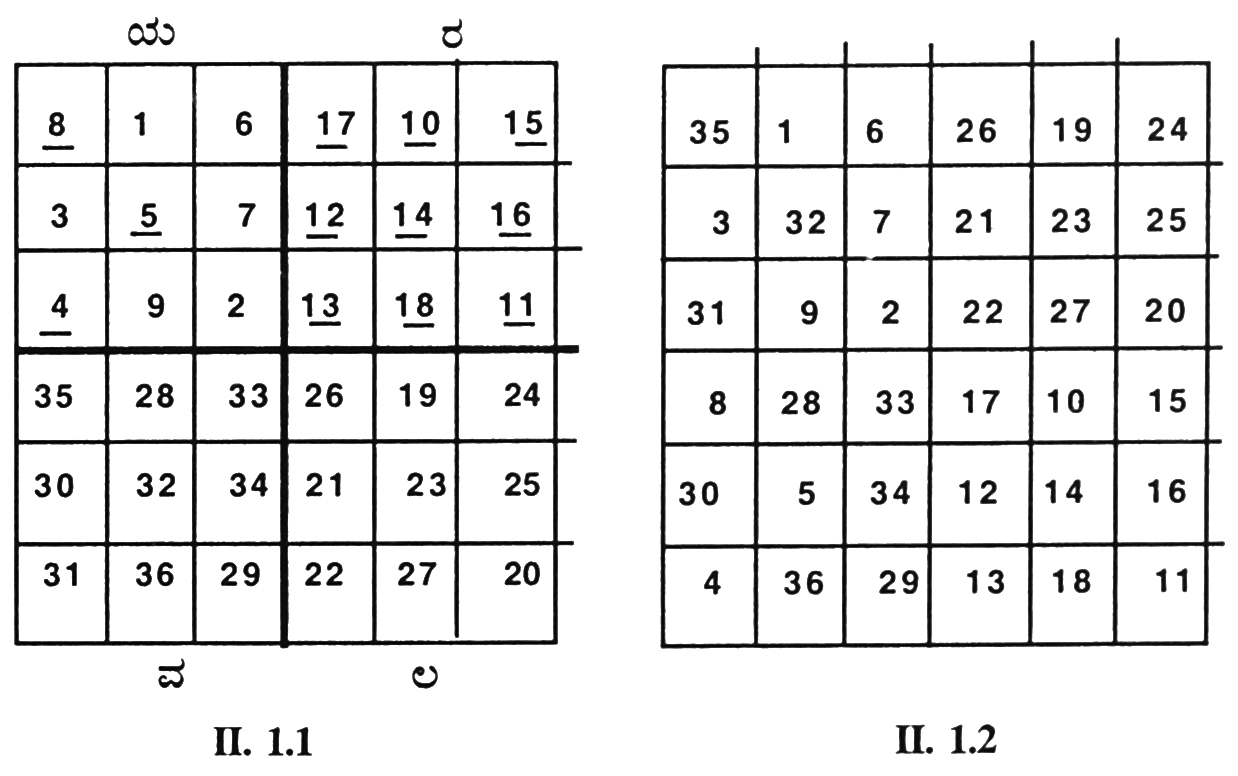
\includegraphics[scale=.97]{src/figures/chap3/fig3-14.jpg}
\end{figure}
\begin{figure}[H]
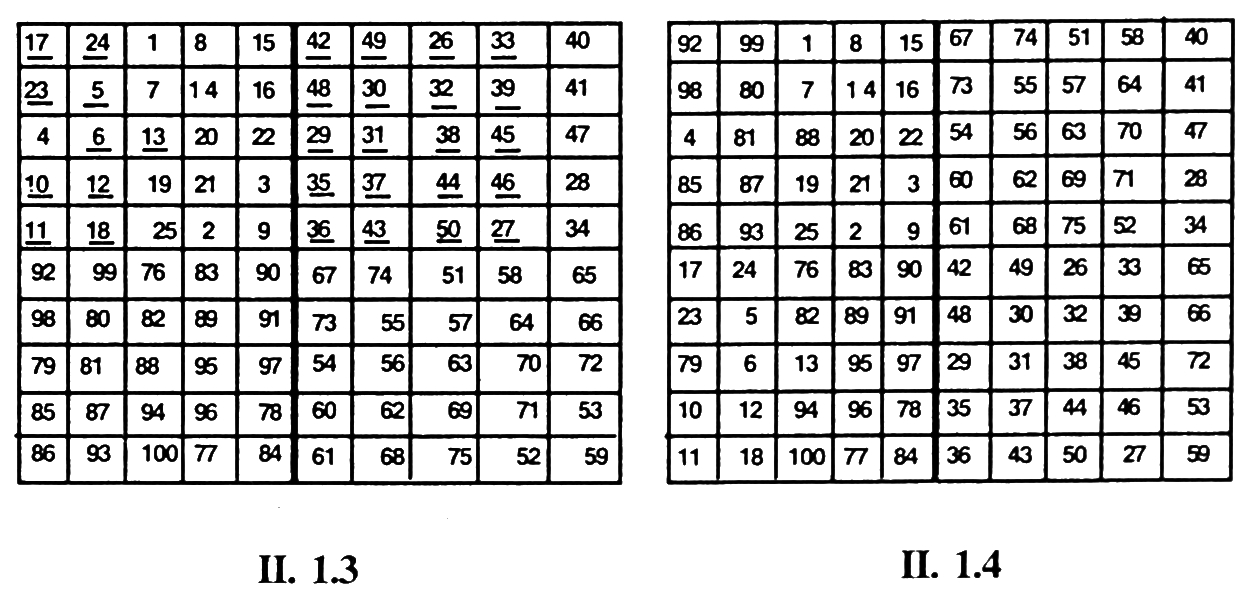
\includegraphics{src/figures/chap3/fig3-15.jpg}
\end{figure}

\begin{itemize}
	\item $n=2$ \{ $2(2n+1)$ (..ಇದರಲ್ಲಿ ಆದೇಶಿಸಿದರೆ, 10 ಬರುತ್ತದೆ.) \}
	\item II.1.3ಯಲ್ಲಿ $10\times 10$ ಚೌಕವನ್ನು 4ಸಮಭಾಗಗಳಾಗಿ ಮಾಡಿದೆ.
	\item ನಾಲ್ಕು ಚೌಕಗಳಲ್ಲೂ 1ರಿಂದ 25, 26-50, 51ರಿಂದ 75, 76--100 ಸಂಖ್ಯೆ ಬಳಸಿ ಮಾಯಾಚೌಕಗಳನ್ನು ರಚಿಸಿದೆ.
	\item ಮೊದಲ ಚೌಕದ ಮಧ್ಯದ ಅಡ್ಡಸಾಲಿನ ಮೊದಲ ಚೌಕ ಹೊರತುಪಡಿಸಿ $‘n’$ ಸಂಖ್ಯೆಯನ್ನು ರೇಖಾಂಕನ ಮಾಡಿದೆ. ಉಳಿದ ಅಡ್ಡಸಾಲುಗಳಲ್ಲಿ $n$ ಸಂಖ್ಯೆಗಳನ್ನು ರೇಖಾಂಕನ ಮಾಡಿದೆ.
	\item ಮೇಲ್ಗಡೆಯ ಎರಡನೇ ಚೌಕದ ಎಲ್ಲ ಅಡ್ಡಸಾಲುಗಳಲ್ಲೂ $n+2$ ಸಂಖ್ಯೆಗಳನ್ನು ರೇಖಾಂಕನ ಮಾಡಿದೆ.
	\item ರೇಖಾಂಕನಗೊಳಿಸಿರುವ ಸಂಖ್ಯೆಗಳನ್ನು 4 ಮತ್ತು 3ನೇ ಚೌಕಗಳ ಅನುರೂಪ ಮನೆಗಳಿಗೆ ಅದಲು ಬದಲು ಮಾಡಿದೆ. ( 1ನೇಚೌಕ ಮತ್ತು 4ನೇ ಚೌಕ, 2ನೇ ಚೌಕ ಮತ್ತು 3ನೇ ಚೌಕ) ಚಿತ್ರ.II.1.4.
	\item ಮಾಯಾಚೌಕ ಲಭ್ಯ ಮೊತ್ತ 505.
\end{itemize}

\textbf{II.(2) $4n$ ರೂಪದ ಸಮಸಂಖ್ಯೆಗಳ ಕ್ರಮವರ್ಗದ ಮಾಯಾಚೌಕ ರಚನೆ :}

$4n$ ರೂಪದ ಸಂಖ್ಯೆಗಳು ಈ ರೀತಿ ಇರುತ್ತವೆ.

\begin{center}
$n=1$ ಆದಾಗ 4\\
$n=2$ ಆದಾಗ 8\\
$n=3$ ಆದಾಗ 12
\end{center}
4,8,12,16,20,24.........................ಇತ್ಯಾದಿ

ಈ ಸಂಖ್ಯೆಗಳನ್ನು ಕ್ರಮವರ್ಗವಾಗಿ ಹೊಂದಿರುವ ಮಾಯಾಚೌಕಗಳ ರಚನೆಯನ್ನು ತಿಳಿಯಲು ಯತ್ನಿಸೋಣ.

\textbf{II. 2.1. ವಿಧಾನ :}

ಉದಾಹರಣೆಗೆ 4ನೇ ಕ್ರಮ ವರ್ಗದ ಮಾಯಾಚೌಕ ರಚನೆ ತಿಳಿಯೋಣ. ತುಂಬಿಸಬೇಕಾದ ಸಂಖ್ಯೆಗಳು 1ರಿಂದ 16ವರೆಗಿನ ಕ್ರಮಾಗತ ಸಂಖ್ಯೆಗಳಾಗಿರಲಿ
\begin{figure}[H]
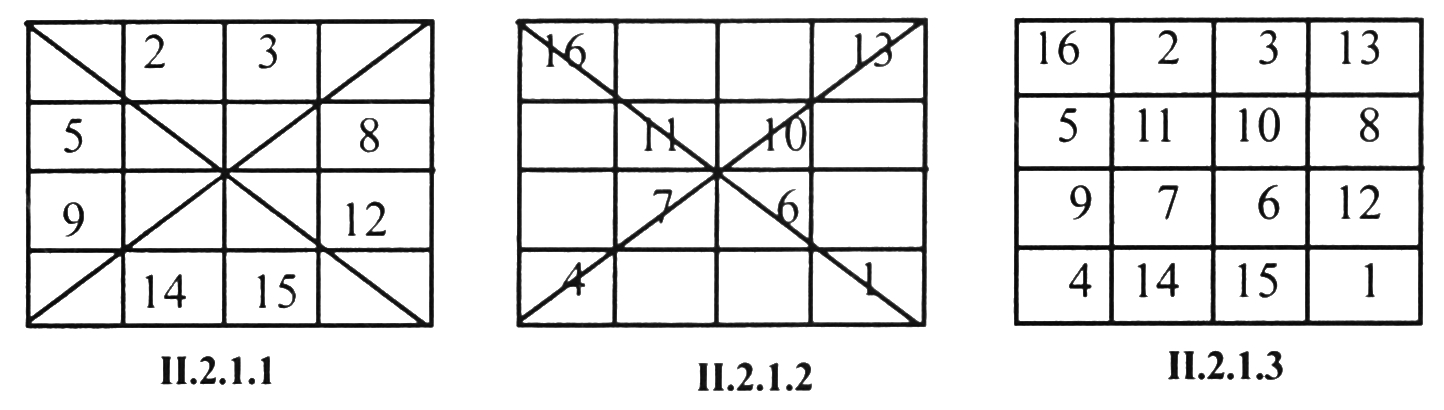
\includegraphics[scale=.9]{src/figures/chap3/fig3-16.jpg}
\end{figure}

\begin{itemize}
	\item $4 \times 4$ ಮನೆಗಳುಳ್ಳ ಮೂರು ಚೌಕಗಳನ್ನು ರಚಿಸಿ. II.2.1.1, II.2.1.2 ಮತ್ತು II.2.1.3 ಆಗಿರಲಿ.
	\item II.2.1.1, ಮತ್ತು II.2.1.2 ಚೌಕಗಳಲ್ಲಿ ಕರ್ಣ ರೇಖೆ ಎಳೆಯಿರಿ.
	\item II.2.1.1 ಚೌಕದಲ್ಲಿ ಎಡಮೇಲ್ತುದಿಯ ಮನೆಯಿಂದ ಪ್ರಾರಂಭಮಾಡಿ. 1ರಿಂದ ಕ್ರಮವಾಗಿ ಎಣಿಸಿ, ಮನೆಗಳನ್ನು ಸಂಖ್ಯೆಗಳಿಂದ ತುಂಬಿಸಿ. ಕರ್ಣರೇಖೆ ಹಾದುಹೋಗಿರುವ ಮನೆಯನ್ನು ಎಣಿಕೆ ಮಾಡಿ, ಆದರೆ ತುಂಬಿಸಬೇಡಿ. ಖಾಲಿ ಮನೆಗಳನ್ನು ಮಾತ್ರ ತುಂಬಿಸಿ. ಚಿತ್ರ II.2.1.1,ನೋಡಿ.
	\item II.2.1.2 ಚೌಕದ ಬಲಕೆಳತುದಿಯ ಮನೆಯಿಂದ ಪ್ರಾರಂಭಿಸಿ 1ರಿಂದ ಕ್ರಮವಾಗಿ ಎಣಿಸಿ, ಕರ್ಣರೇಖೆ ಹಾದು ಹೋಗಿರುವ ಮನೆಗಳನ್ನು ತುಂಬಿಸಿ. ಖಾಲಿ ಮನೆಗಳನ್ನು ಎಣಿಸಿ, ಆದರೆ ತುಂಬಿಸಬೇಡಿ. ಚಿತ್ರ II.2.1.2 ನೋಡಿ, ಮನೆಗಳನ್ನು ಬಲದಿಂದ ಎಡಕ್ಕೆ ಎಣಿಸಿ, ತುಂಬಿಸಿ.
	\item II.2.1.3 ಚೌಕದಲ್ಲಿ ಉಳಿದೆರಡು ಚೌಕಗಳಲ್ಲಿರುವ ಸಂಖ್ಯೆಗಳನ್ನು ಅನುರೂಪ ಮನೆಗಳಲ್ಲಿ ತುಂಬಿಸಿ. ಲಭಿಸುವುದು 4ನೇ ಕ್ರಮವರ್ಗದ ಮಾಯಾಚೌಕ ಮೊತ್ತ 34.
\end{itemize}

1ರಿಂದ 16 ಕ್ರಮಾಗತ ಸಂಖ್ಯೆಗಳ ಬದಲು ಯಾವುದೇ ಅಂಕಗಣಿತ ಶ್ರೇಢಿಯ ಕ್ರಮವಾದ 16 ಸಂಖ್ಯೆಗಳನ್ನು ಆಯ್ಕೆಮಾಡಿಕೊಳ್ಳಬಹುದು.

ಇನ್ನೊಂದು ಉದಾಹರಣೆಯನ್ನು ನೋಡೋಣ.

$8 \times 8$ ಮಾಯಾಚೌಕ. 1ರಿಂದ 64ರವರೆಗೆ ಕ್ರಮಾಗತ ಸಂಖ್ಯೆಗಳು.
\begin{figure}[h]
\includegraphics{src/figures/chap3/fig3-17.eps}\\
\caption*{II.2.1.4}
\end{figure}
\begin{figure}[h]
\includegraphics{src/figures/chap3/fig3-18.eps}\\
\caption*{II.2.1.5}
\end{figure}

\begin{itemize}
	\item ಎರಡು $8 \times 8$ ಚೌಕಗಳನ್ನು ರಚಿಸಿ. II.2.1.4, II.2.1.5
	\item II.2.1.4 ಚೌಕವನ್ನು $4 \times 4$ಚೌಕಗಳ ನಾಲ್ಕು ಸಮಭಾಗಗಳಾಗಿ ಮಾಡಿ.

	ಎಲ್ಲ ಭಾಗಗಳಿಗೂ ಕರ್ಣಗಳನ್ನು ಎಳೆಯಿರಿ.
	\item II.2.1.4 ಚೌಕದ ಎಡ ಮೇಲ್ತುದಿಯ ಮನೆಯಿಂದ ಪ್ರಾರಂಭಿಸಿ 1,2,3,4.....ಎಣಿಕೆ ಮಾಡುತ್ತಾ, ಕರ್ಣ ಹಾದು ಹೋಗದೇ ಇರುವ ಮನೆಗಳನ್ನು ಎಣಿಕೆಯಲ್ಲಿ ಅವುಗಳಿಗೆ ಬರುವ ಸಂಖ್ಯೆಗಳಿಂದ ತುಂಬಿಸಿ. II.ಚಿತ್ರ..2.1.4
	\item II.2.1.4 ಚಿತ್ರದಲ್ಲಿ ತುಂಬಿಸಿರುವ ಸಂಖ್ಯೆಗಳನ್ನು II.2.1.5 ಚೌಕದ ಅನುರೂಪ ಮನೆಗಳಿಗೆ ವರ್ಗಾಯಿಸಿ ಬರೆಯಿರಿ.
	\item II.2.1.5 ಚೌಕದ ಕೆಳಗಿನ ಕೊನೆಯ ಅಡ್ಡಸಾಲಿನ ಬಲಗಡೆ ಕೊನೆ ಮನೆಯಿಂದ ಪ್ರಾರಂಭಿಸಿ, 1,2,3,4...........ಎಣಿಕೆ ಮಾಡುತ್ತಾ, ಸಂಖ್ಯೆಗಳಿಲ್ಲದ (ಕರ್ಣರೇಖೆ ಇರುತ್ತದೆ) ಮನೆಗಳನ್ನು ಕ್ರಮವಾಗಿ ತುಂಬಿಸಿ. ಈಗಾಗಲೇ ಸಂಖ್ಯೆಗಳಿರುವ ಮನೆಗಳನ್ನು ಎಣಿಕೆಗೆ ತೆಗೆದುಕೊಳ್ಳಿ. ಪ್ರತಿ ಅಡ್ಡಸಾಲನ್ನು ಬಲದಿಂದ ಎಡಕ್ಕೆ ಗಮಿಸುತ್ತಾ ತುಂಬಿಸಿ. ಈ ಚೌಕದಲ್ಲಿ ಕರ್ಣಗಳು ಬರುವ ಮನೆಗಳನ್ನು ಮಸುಕು ಮಾಡಿದೆ. (Shaded)
	\item II.2.1.5 ಇದು 8ನೇ ಕ್ರಮವರ್ಗದ ಮಾಯಾಚೌಕ. ಮೊತ್ತ 260.

	ಮತ್ತೊಂದು ಉದಾಹರಣೆ 12ನೇ ಕ್ರಮವರ್ಗದ ಮಾಯಾಚೌಕ ರಚನೆ. $12\times 12$ ರ ಚೌಕವನ್ನು $4 \times 4$ ರ ಚೌಕಗಳಾಗಿ ವಿಭಾಗಿಸಿ ಕರ್ಣರೇಖೆಗಳನ್ನು ಎಳೆಯಿರಿ. ಹಿಂದೆ ಹೇಳಿರುವ ರೀತಿಯಲ್ಲಿ ಸಂಖ್ಯೆಗಳನ್ನು ತುಂಬಿಸಿ. ಚಿತ್ರ II.2.1.6
	\begin{figure}[h]
	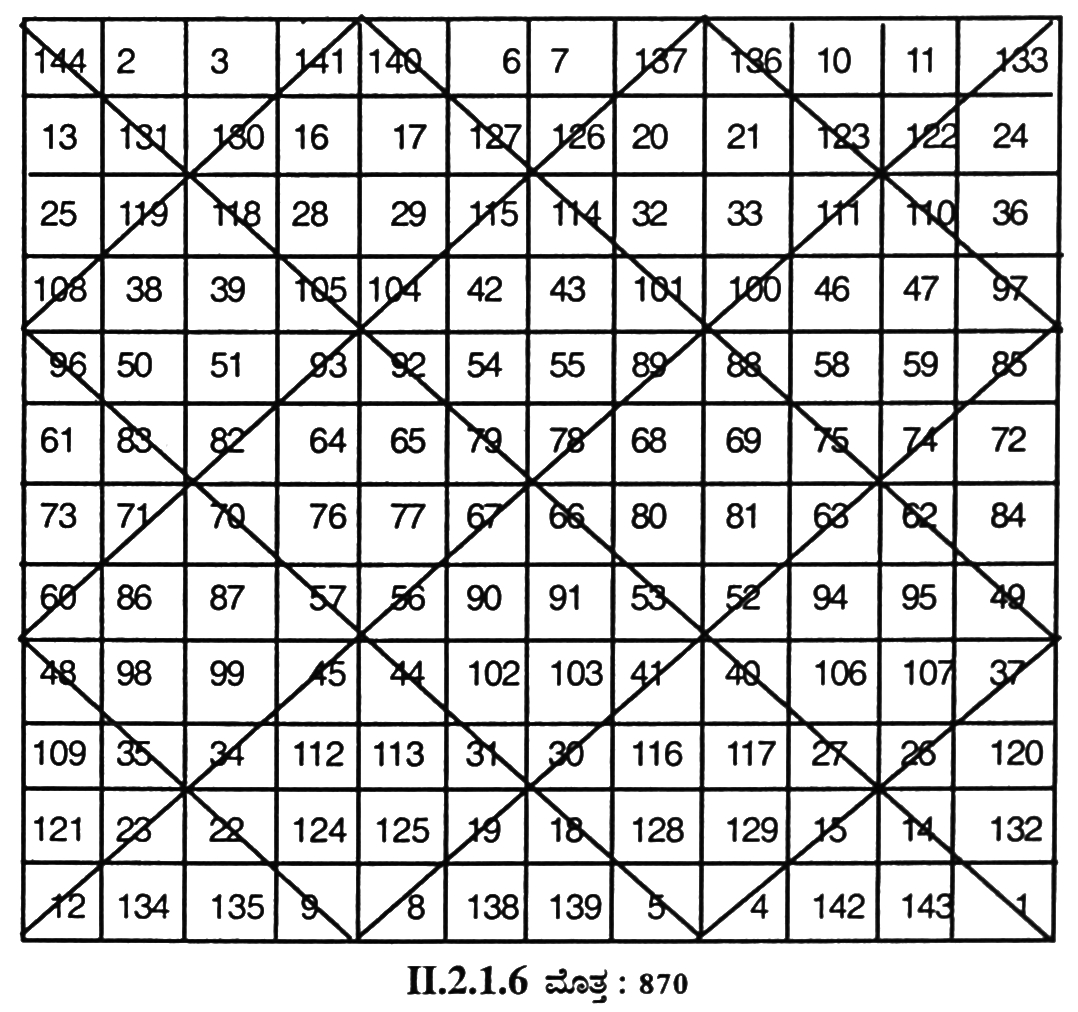
\includegraphics{src/figures/chap3/fig3-19.jpg}
	\end{figure}
\end{itemize}

\textbf{ವಿಧಾನ : II.2.2.}

ಉದಾಹರಣೆ : 8ನೇ ಕ್ರಮವರ್ಗದ ಮಾಯಾಚೌಕದ ರಚನೆ

1 ರಿಂದ 64ರ ವರೆಗಿನ ಕ್ರಮಾಗತ ಸಂಖ್ಯೆಗಳು

\textbf{ಹಂತಗಳು :}
\begin{itemize}
	\item $8 \times 8$ ಮನೆಗಳಿರುವ 4 ಚೌಕಗಳನ್ನು ರಚಿಸಿ. ಚಿತ್ರ II.2.2.1,ಚಿತ್ರ II.2.2.2 ಚಿತ್ರ II.2.2.3 ಮತ್ತು ಚಿತ್ರ II.2.2.4ಆಗಿರಲಿ.
	\item II.2.2.1 ಚೌಕದಲ್ಲಿ 1ರಿಂದ 64ರವರೆಗಿನ ಸಂಖ್ಯೆಗಳನ್ನು ಮೊದಲ ಅಡ್ಡಸಾಲಿನ ಮೊದಲ ಮನೆಯಿಂದ ಪ್ರಾರಂಭಿಸಿ ಚೌಕದ ಎಲ್ಲ ಮನೆಗಳನ್ನು ಕ್ರಮವಾಗಿ ತುಂಬಿಸಿ.
	\item II.2.2.1,ಚೌಕದಲ್ಲಿನ ಕರ್ಣಗಳ ಮನೆಗಳಲ್ಲಿರುವ ಸಂಖ್ಯೆಗಳನ್ನು ತಿರುವು ಮುರುವು ಮಾಡಿ. ಅಂದರೆ 1,10,19,.....55,64 ಇರುವುದನ್ನು 64,55....19.10,1 ಆಗುವಂತೆ - ಅದೇ ಕರ್ಣದ ಮನೆಗಳಲ್ಲಿ ತುಂಬಿಸಿ. ಇನ್ನೊಂದು ಕರ್ಣವನ್ನು ಹೀಗೆಯೇ ತಿರುವು ಮುರುವು ಮಾಡಿ ಬರೆಯಿರಿ. ಉಳಿದ ಕರ್ಣೋತ್ತರ ಮನೆಗಳಲ್ಲಿನ ಸಂಖ್ಯೆಗಳನ್ನು ಅವುಗಳ ಮನೆಗಳಲ್ಲಿಯೇ ಬರೆಯಿರಿ. ಚಿತ್ರ II.2.2.2
	\item II.2.2.2 ಚೌಕವನ್ನು ಮೇಲಿನಿಂದ ಕೆಳಕ್ಕೆ ಎರಡು ಸಮಭಾಗವಾಗಿ ವಿಭಾಗಿಸಿ. ಪ್ರತಿಭಾಗದಲ್ಲಿಯೂ $4 \times 8$ ಮನೆಗಳಿರುತ್ತವೆ.
	\item II.2.2.2 ಚೌಕದ ಬಲ ಅರ್ಧ $4 \times 8$ ಚೌಕದಲ್ಲಿರುವ ಸಂಖ್ಯೆಗಳನ್ನು II.2.2.3 ಚೌಕದ ಎಡ ಅರ್ಧ ಭಾಗದ ಮನೆಗಳಲ್ಲಿಯೂ, ಎಡ ಅರ್ಧ $4 \times 8$ ಚೌಕದಲ್ಲಿರುವ ಸಂಖ್ಯೆಗಳನ್ನು II.2.2.3 ಚೌಕದ ಬಲ ಅರ್ಧ $4 \times 8$ ಚೌಕದ ಮನೆಗಳಲ್ಲಿಯೂ ತುಂಬಿಸಿ. ಚಿತ್ರ II.2.2.3
	\item II.2.2.3 ಚೌಕದ ಎರಡು ಕರ್ಣಗಳ ಸಂಖ್ಯೆಗಳನ್ನೂ ತಿರುವು ಮುರುವು ಮಾಡಿ II.2.2.4 ಚೌಕದ ಕರ್ಣಮನೆಗಳಲ್ಲಿ ಕ್ರಮವಾಗಿ ತುಂಬಿಸಿ. II.2.2.3 ಚೌಕದ ಕರ್ಣೇತರ ಮನೆಗಳಲ್ಲಿನ ಸಂಖ್ಯೆಗಳನ್ನು II.2.2.4 ಚೌಕದಲ್ಲಿ ಅನುರೂಪ ಮನೆಗಳಲ್ಲಿ ತುಂಬಿಸಿ. ಚಿತ್ರ II.2.2.4 ನೋಡಿ.

	ಲಭಿಸಿರುವುದು ಮಾಯಾಚೌಕ. ಮೊತ್ತ 260
	\begin{figure}[H]
	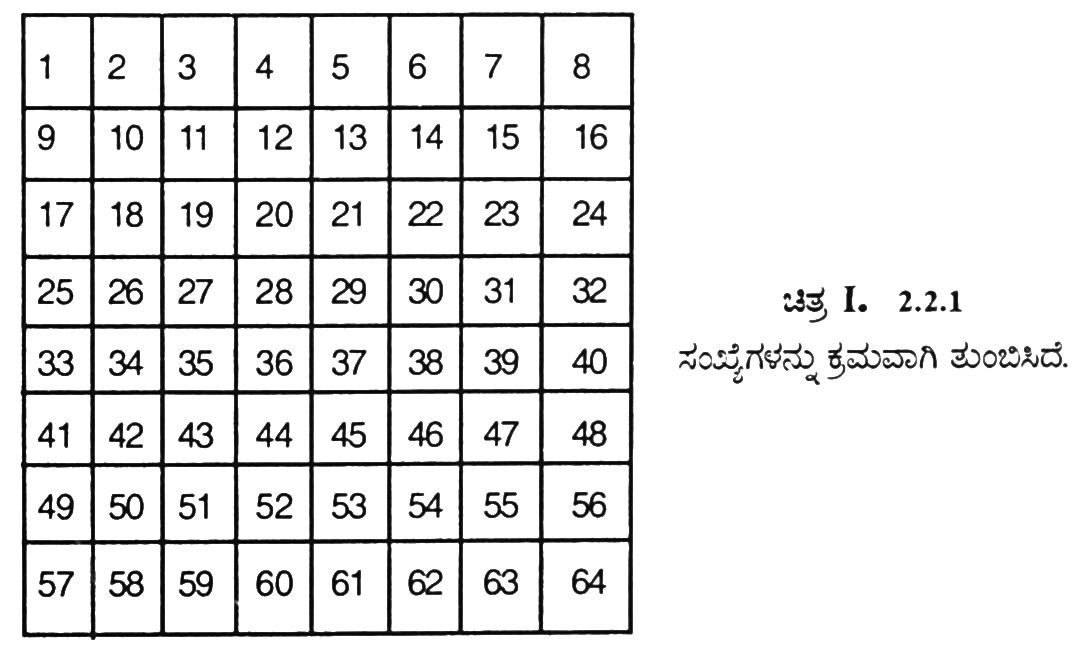
\includegraphics[scale=1.18]{src/figures/chap3/fig3-20.jpg}
	\end{figure}
	\begin{figure}[H]
	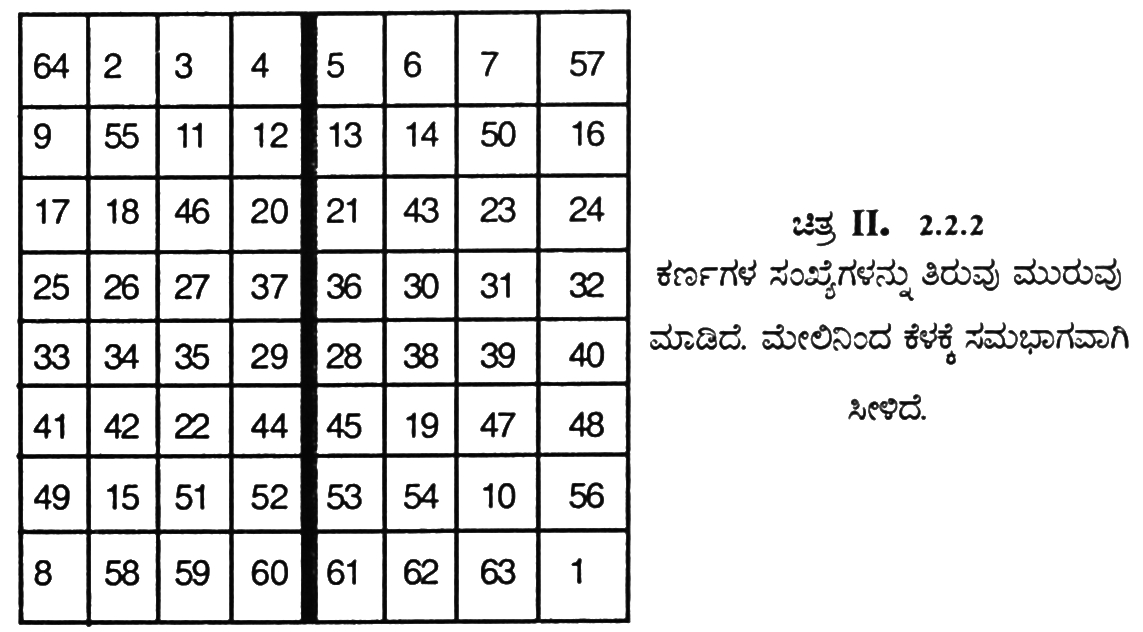
\includegraphics[scale=.92]{src/figures/chap3/fig3-21.jpg}
	\end{figure}
	\begin{figure}[H]
	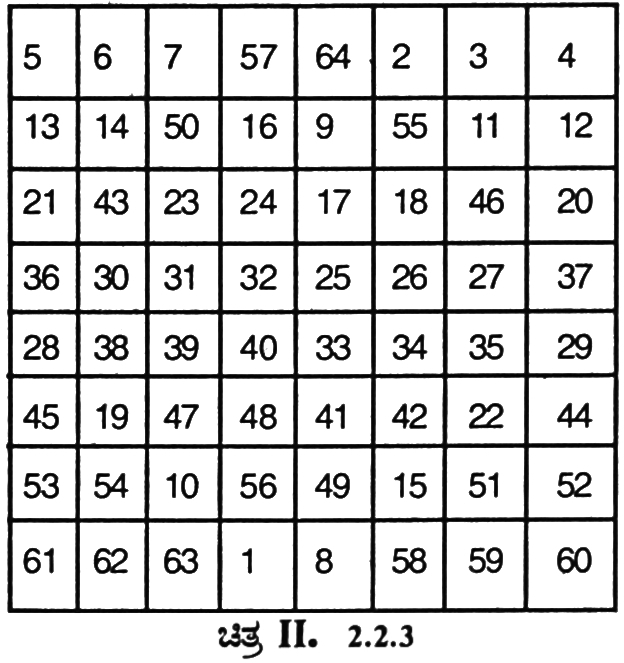
\includegraphics[scale=.92]{src/figures/chap3/fig3-22.jpg}
	\end{figure}
	\begin{figure}[H]
	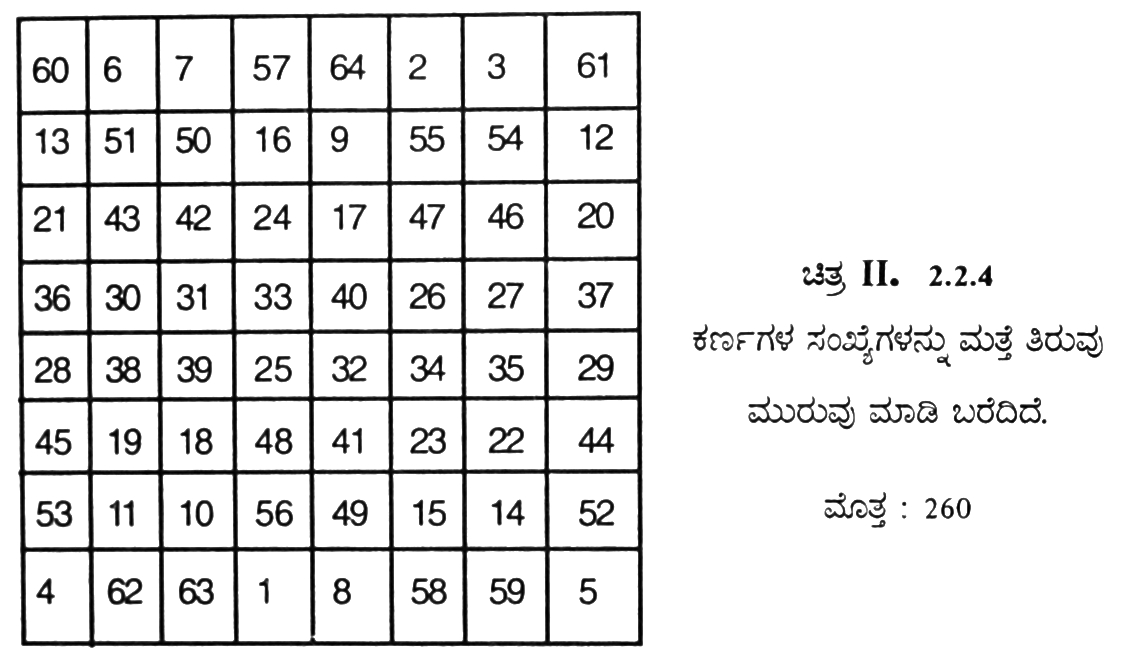
\includegraphics[scale=.92]{src/figures/chap3/fig3-23.jpg}
	%\caption{ಚಿತ್ರ II. 2.2.4 \\ ಕರ್ಣಗಳ ಸಂಖ್ಯೆಗಳನ್ನು ಮತ್ತೆ ತಿರುವು ಮುರುವು ಮಾಡಿ ಬರೆದಿದೆ. \\ ಮೊತ್ತ : 260}
	\end{figure}
\end{itemize}
\textbf{ವಿಧಾನ II. 2.3.}

$4n$ ರೂಪದ ಸಮಸಂಖ್ಯೆ ಕ್ರಮವರ್ಗದ ಮಾಯಾಚೌಕ ರಚನೆಗೆ ಎರಡು ವಿಧಾನಗಳನ್ನು ತಿಳಿದಿದ್ದೇವೆ. ಮತ್ತೊಂದು ವಿಧಾನ ಕಲಿಯೋಣ.

ಉದಾ: $8 \times 8$ ಮಾಯಾಚೌಕ ; ಸಂಖ್ಯೆಗಳು 1,2,3....64.

\textbf{ಹಂತಗಳು :-}
\begin{itemize}
	\item $8 \times 8$ ಮನೆಗಳುಳ್ಳ ನಾಲ್ಕು ಚೌಕಗಳನ್ನು ರಚಿಸಿ. II.2.3.1, II.2.3.2, II.2.3.3 ಮತ್ತು II. 2.3.4
	\item II.2.3.1 ಚೌಕದಲ್ಲಿ 1ರಿಂದ 64ರ ವರೆಗೆ ಸಂಖ್ಯೆಗಳನ್ನು ಎಡ ಮೇಲ್ತುದಿಯ ಮನೆಯಿಂದ ಪ್ರಾರಂಭಿಸಿ, ಬಲ ಕೆಳತುದಿಯ ಮನೆಯವರೆಗೆ ಕ್ರಮವಾಗಿ ತುಂಬಿಸಿ.
	\item II.2.3.1 ಚೌಕವನ್ನು ನಾಲ್ಕು ಸಮಭಾಗಗಳಾಗಿ ವಿಭಾಗಿಸಿ. ಪ್ರತಿಯೊಂದು $4 \times 4$ ಚೌಕಗಳಾಗಿರುತ್ತವೆ. ಇವುಗಳಿಗೆ $a, b, c, d$ ಹೆಸರಿಸಿ. (ಪ್ರದಕ್ಷಿಣವಾಗಿ)
	\item $4 \times 4$ರ ಪ್ರತಿ ಚೌಕವನ್ನು $2 \times 2$ರ ನಾಲ್ಕು ಚೌಕಗಳಾಗಿ ವಿಭಾಗಿಸಿ. ಒಟ್ಟು 16 ಚೌಕಗಳಿರುತ್ತವೆ. a ಭಾಗದಲ್ಲಿರುವ ನಾಲ್ಕು $2 \times 2$ ಚೌಕಗಳಿಗೆ $a_1, a_2, a_3, a_4$ ಎಂದು ಹೆಸರಿಸಿ $2 \times 2$ ಚೌಕದ ಮಧ್ಯದಲ್ಲಿ ಬರೆಯಿರಿ. ಇದೇ ರೀತಿ b, c, ಮತ್ತು d ಚೌಕಗಳನ್ನು ವಿಭಾಗಿಸಿ. $b_1, b_2, c_3, d_4$, ಮತ್ತು $d_1, d_2, d_3, d_4$ ಹೆಸರುಗಳನ್ನು ಕೊಡಿ. ಚಿತ್ರ.II.2.3.1. ನೋಡಿ.

	\item $a_1, a_3$, ಚೌಕಗಳಲ್ಲಿನ ಸಂಖ್ಯೆಗಳನ್ನು ಅವುಗಳ ಕೇಂದ್ರ ಪ್ರತಿಬಿಂಬ ಸ್ಥಾನ (Skew) ಚೌಕಗಳಾದ $c_3, c_1$, ಚೌಕಗಳ ಸಂಖ್ಯೆಗಳೊಡನೆ ಅದಲು ಬದಲು ಮಾಡಿ ಬರೆಯಿರಿ. ಇದೇ ರೀತಿ $b_2, b_4$, ಚೌಕಗಳಲ್ಲಿನ ಸಂಖ್ಯೆಗಳನ್ನು $d_1, d_3$,ಚೌಕಗಳಲ್ಲಿನ ಸ್ಕ್ಯೂ  ಸಂಖ್ಯೆಗಳೊಡನೆ ಅದಲು ಬದಲು ಮಾಡಿ ಬರೆಯಿರಿ. ಚಿತ್ರ. II.2.3.2. ನೋಡಿ.
	\item $a_2, a_4$; $b_1, b_3$; $c_2, c_4$; $d_1, d_3$, ಚೌಕಗಳಲ್ಲಿನ ಸಂಖ್ಯೆಗಳು ಸ್ಥಾನ ಬದಲಾವಣೆ ಹೊಂದುವುದಿಲ್ಲ. ಅವುಗಳನ್ನು ಸ್ಥಾನದಲ್ಲಿಯೇ ಚಿತ್ರ. II.2.3.3 ಚೌಕದಲ್ಲಿ ಬರೆಯಿರಿ.
	\item II.2.3.2 ಮತ್ತು II.2.3.3 ಚೌಕಗಳಲ್ಲಿ ಬರೆದಿರುವ ಸಂಖ್ಯೆಗಳನ್ನು II.2.3.4 ಚೌಕದಲ್ಲಿ ಅನುರೂಪ (Corresponding) ಮನೆಗಳಿಗೆ ವರ್ಗಾಯಿಸಿ. ಇದು ಮಾಯಾಚೌಕ. ಮೊತ್ತ 260.
\end{itemize}

ಇದೇ ರೀತಿ 12 ಕ್ರಮವರ್ಗದ ಮಾಯಾಚೌಕವನ್ನು ರಚಿಸಬಹುದು. ಈ ಕೆಳಗೆ ರಚಿಸಿ ತೋರಿಸಲಾಗಿದೆ. 16, 20 ಇತ್ಯಾದಿ ಕ್ರಮವರ್ಗದ ಮಾಯಾಚೌಕಗಳನ್ನು ರಚಿಸಿ, ಆನಂದ ಪಡಿ.
\begin{figure}[H]
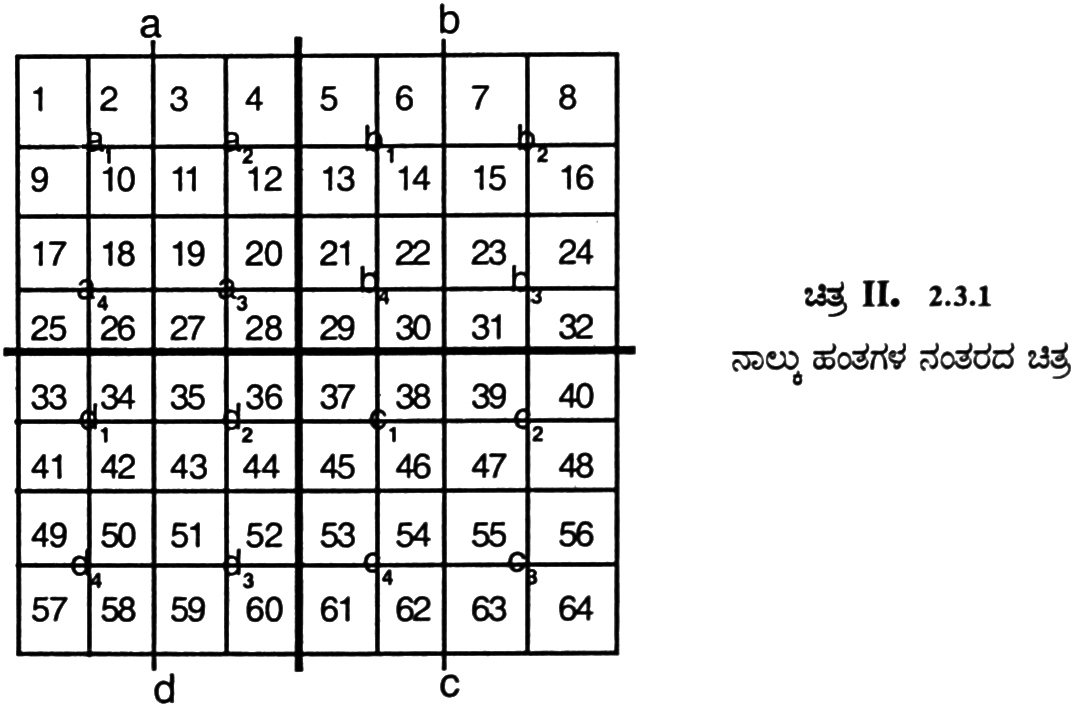
\includegraphics[scale=.9]{src/figures/chap3/fig3-24.jpg}
\end{figure}
\begin{figure}[H]
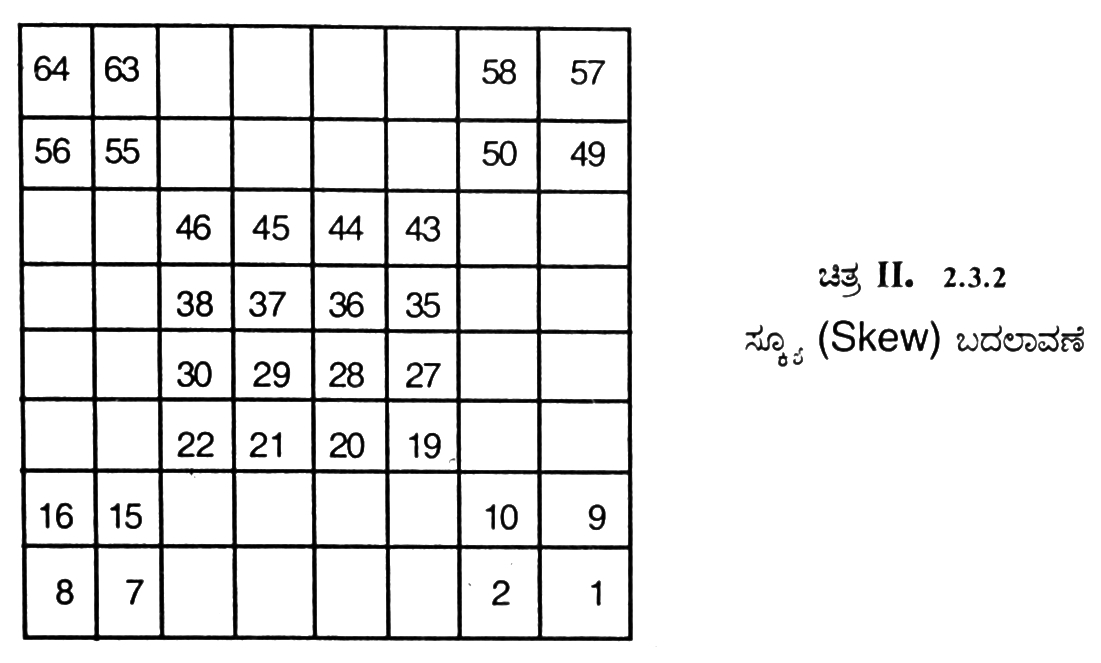
\includegraphics[scale=.85]{src/figures/chap3/fig3-25.jpg}
\end{figure}
\begin{figure}[H]
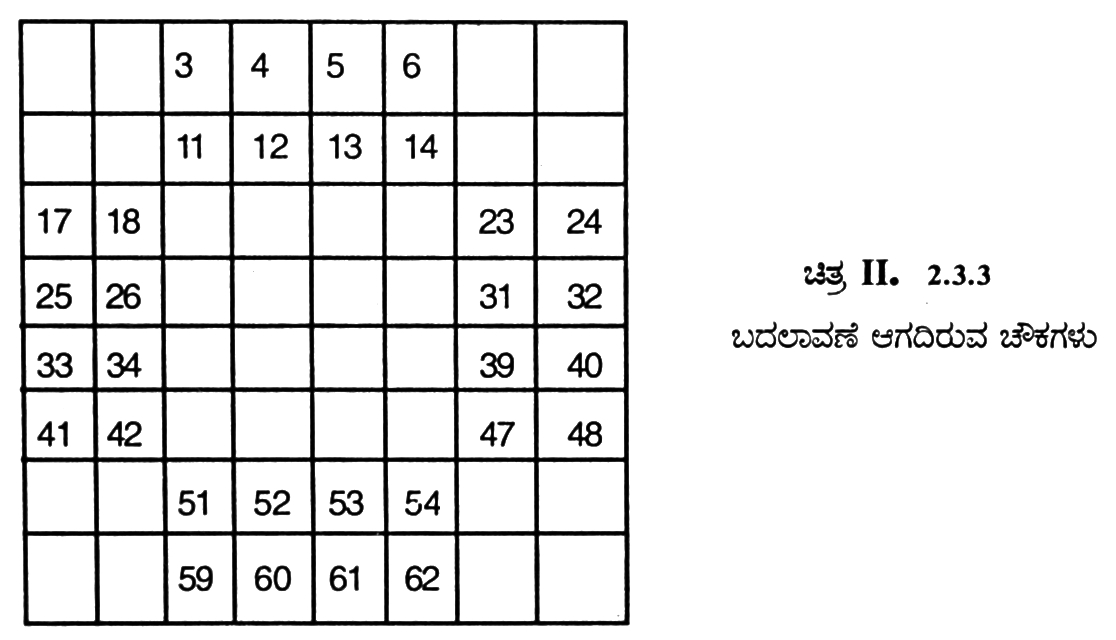
\includegraphics[scale=.9]{src/figures/chap3/fig3-26.jpg}
\end{figure}
\begin{figure}[H]
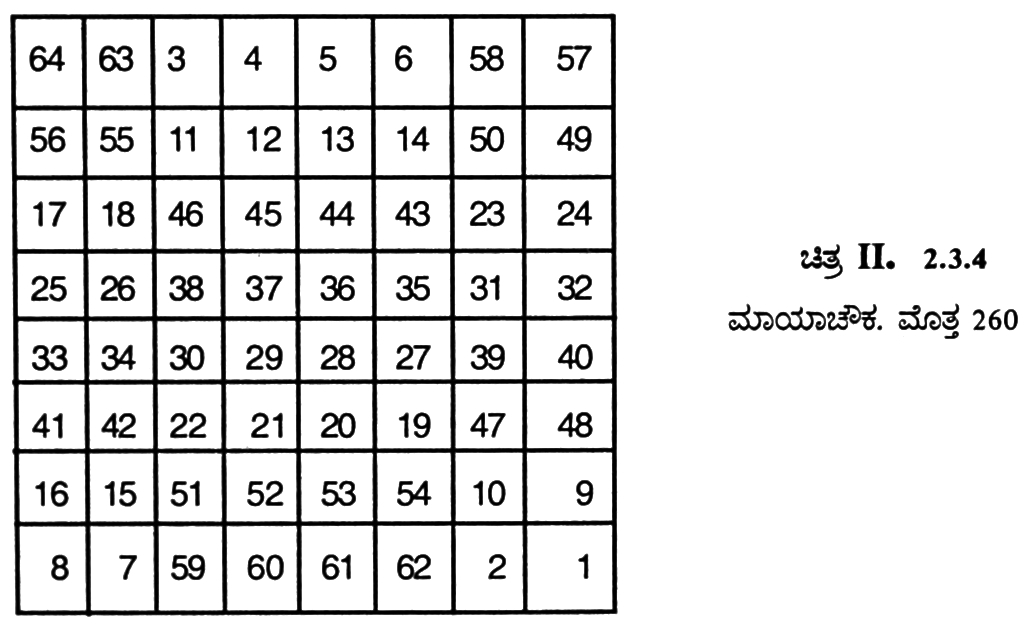
\includegraphics{src/figures/chap3/fig3-27.jpg}
\end{figure}
ಇದೇ ವಿಧಾನದಲ್ಲಿ 12 ಕ್ರಮವರ್ಗದ ಮಾಯಾಚೌಕ ರಚಿಸಿದೆ. ಮೊತ್ತ 870
\begin{figure}[H]
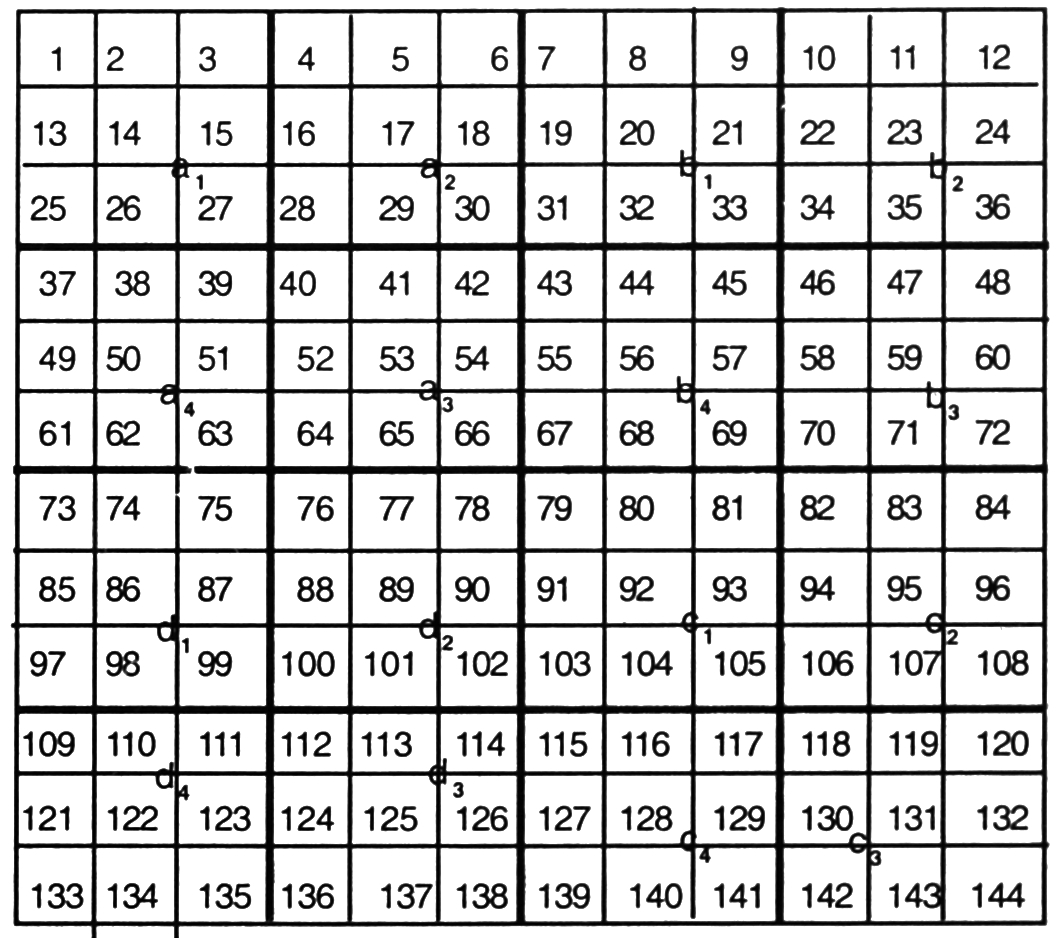
\includegraphics[scale=.9]{src/figures/chap3/fig3-28.jpg}
\end{figure}
\begin{figure}[H]
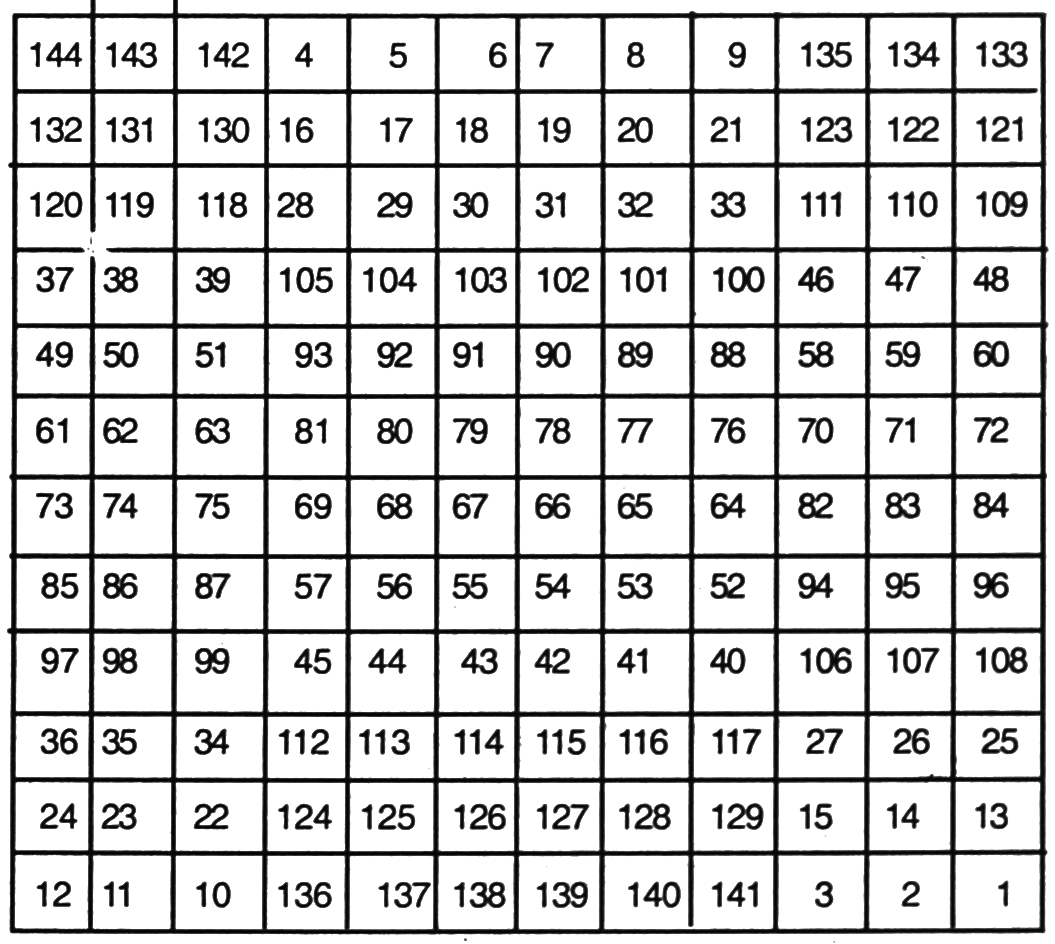
\includegraphics[scale=.9]{src/figures/chap3/fig3-29.jpg}
\end{figure}

\textbf{ವಿಧಾನ III. ಗುಚ್ಛ ಮಾಯಾಚೌಕಗಳ ವಿಧಾನ :}

ಹೂ ಗುಚ್ಛಗಳನ್ನು (bouquet) ನೋಡಿದ್ದೀರಲ್ಲವೇ? ಬೇರೆ ಬೇರೆ ಬಣ್ಣಗಳ, ವಿವಿಧ ಆಕಾರಗಳ ಪುಷ್ಪಗಳನ್ನು ಆಕರ್ಷಕವಾಗುವಂತೆ ಜೋಡಿಸಿರುತ್ತಾರಲ್ಲವೇ? ಇಂತಹ ಗುಚ್ಛಗಳು ನೋಡುಗರ ಮನಸ್ಸಿಗೆ ಮುದ ನೀಡುತ್ತವೆಯಲ್ಲವೇ? ಹೀಗೆಯೇ ಮಾಯಾ ಚೌಕಗಳನ್ನು ನಿರ್ದಿಷ್ಟ ರೀತಿಯಲ್ಲಿ ಜೋಡಣೆ ಮಾಡಿದಾಗ ಮಾಯಾಚೌಕಗಳ ಗುಚ್ಛ ಅಥವಾ ಗುಚ್ಛ ಮಾಯಾಚೌಕ (Composite or Cluster Magic square) ದೊರೆಯುತ್ತದೆ.

ಇಂತಹ ಗುಚ್ಛ ಮಾಯಾಚೌಕ ರಚನೆಯನ್ನು ತಿಳಿಯೋಣ. ಹೆಸರೇ ಹೇಳುವಂತೆ ಇದರಲ್ಲಿ ಮಾಯಾಚೌಕಗಳ ಗುಚ್ಛ ಅಥವಾ ಗುಂಪು ಇರುತ್ತದೆ. 3,4 ಮತ್ತು 5 ಕ್ರಮವರ್ಗಗಳ ಮಾಯಾಚೌಕಗಳನ್ನು ನಿರ್ದಿಷ್ಟ ಕ್ರಮದಲ್ಲಿ ಜೋಡಿಸಿ ಬರೆದರೆ ಲಭಿಸುವುದು ಒಂದು ಮಾಯಾಚೌಕವೇ. 3,4 ಮತ್ತು 5 ಇವುಗಳ ಗುಣಕ ಸಂಖ್ಯೆಗಳ ಕ್ರಮವರ್ಗದ ಮಾಯಾಚೌಕ ಗಳನ್ನು ರಚಿಸಲು ಈ ವಿಧಾನ ಸಹಾಯಕ. ಗುಣಕಗಳು ಎಂದರೆ. ($3 \times 3=9$, $3 \times 4=12$, $3 \times 5=15$, $4 \times 5= 20$, $4 \times 4=16$, ಇತ್ಯಾದಿ) 9,12,15,16,20........ ಸಂಖ್ಯೆಗಳು, ಈ ಸಂಖ್ಯೆಗಳ ಕ್ರಮವರ್ಗದ ಮಾಯಾಚೌಕಗಳನ್ನು ರಚಿಸಲು ಈಗಾಗಲೇ ಕೆಲವು ವಿಧಾನಗಳನ್ನು ಚರ್ಚಿಸಲಾಗಿದೆ. ಆದರೂ ಗುಚ್ಛ ವಿಧಾನದಲ್ಲಿ ರಚಿಸುವುದು ಖುಷಿ ತರುವಂತಹುದು. ಹಾಗಾಗಿ ಈ ವಿಧಾನವನ್ನು ಪರಿಶೀಲಿಸೋಣ.

ಈ ವಿಧಾನದಲ್ಲಿ ಮಾಯಾಚೌಕ ರಚಿಸಲು ಅತ್ಯಗತ್ಯವೆಂದರೆ, 3,4 ಮತ್ತು 5 ಕ್ರಮವರ್ಗಗಳ ಮಾಯಾಚೌಕಗಳ ಪೂರ್ಣ ಪರಿಚಯ. ಇವುಗಳಲ್ಲಿ 1ರಿಂದ ಪ್ರಾರಂಭಿಸಿ ಕ್ರಮಾಗತ ಸಂಖ್ಯೆಗಳಿಂದ ಮಾಯಾಚೌಕ ರಚಿಸಿದಾಗ ಅವುಗಳಲ್ಲಿ ಬರುವ ಸಂಖ್ಯಾಸ್ಥಾನಗಳ ಸ್ಪಷ್ಟ ಅರಿವು ಅವಶ್ಯಕ.
\begin{figure}[h]
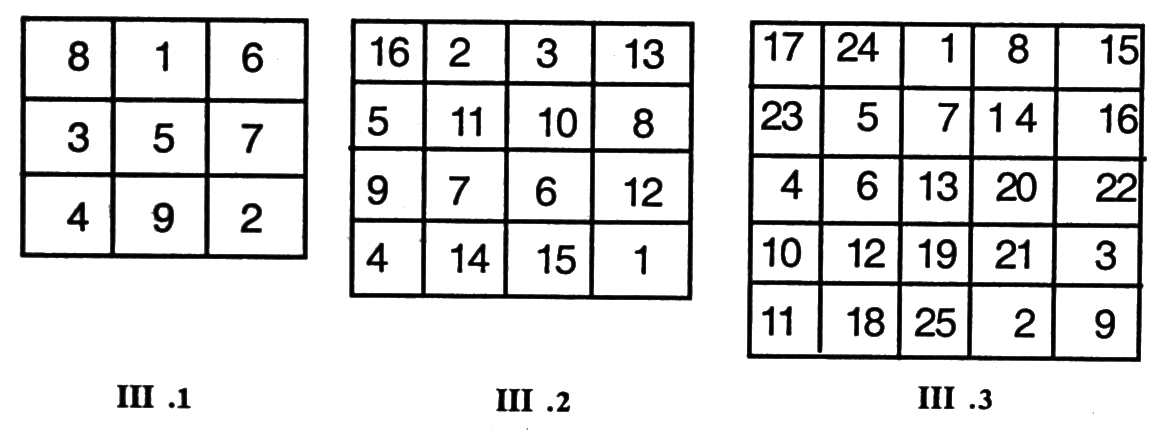
\includegraphics{src/figures/chap3/fig3-30.jpg}
\end{figure}

ಈಗ 9ನೇ ಕ್ರಮವರ್ಗದ ಮಾಯಾಚೌಕವನ್ನು ಈ ವಿಧಾನದಲ್ಲಿ ರಚಿಸೋಣ.

\textbf{ಹಂತಗಳು :}
\begin{itemize}
	\item $9 \times 9$ ರ ಒಂದು ಚೌಕ ರಚಿಸಿ
	\item ಇದನ್ನು $3 \times 3$ರಚೌಕಗಳಾಗುವಂತೆ 9 ಸಮಭಾಗಗಳಾಗಿ ಮಾಡಿ. ಪ್ರತಿಯೊಂದ ರಲ್ಲಿಯೂ 9 ಮನೆಗಳಿವೆ.
	\item ಮೇಲ್ಗಡೆಯ ಅಡ್ಡಸಾಲಿನ $3 \times 3$ರಚೌಕಗಳಲ್ಲಿ ಮಧ್ಯದ ಚೌಕದಲ್ಲಿ 1ರಿಂದ 9ರ ವರೆಗಿನ ಸಂಖ್ಯೆಗಳನ್ನು ಚಿತ್ರ III.1ರಲ್ಲಿರುವಂತೆ ತುಂಬಿಸಿ, ಮಾಯಾಚೌಕ ರಚಿಸಿ,
	\item ಕೊನೆಯ ಅಡ್ಡಸಾಲಿನ ಕೊನೆಯಲ್ಲಿ ಬರುವ $3 \times 3$ರಚೌಕದಲ್ಲಿ 10ರಿಂದ 18ರವರೆಗಿನ ಸಂಖ್ಯೆಗಳನ್ನು ಬಳಸಿ I.3 ವಿಧಾನದಲ್ಲಿ ಮಾಯಾಚೌಕ ರಚಿಸಿ.
	\item ಈ ಎರಡು ಮಾಯಾಚೌಕಗಳು ಚಿತ್ರ III.1ರಲ್ಲಿ 1 ಮತ್ತು 2 ಬರುವ ಸ್ಥಾನಗಳಲ್ಲಿರುವುದನ್ನು ಗಮನಿಸಿ.
	\item ಹೀಗೆಯೇ 19ರಿಂದ 27, 28 ರಿಂದ 36, 37ರಿಂದ 45, 46ರಿಂದ54, 55ರಿಂದ 63, 64ರಿಂದ 72, ಮತ್ತು 73ರಿಂದ 81, ಸಂಖ್ಯೆಗಳನ್ನು ಬಳಸಿ, $3 \times 3$ರಮಾಯಾಚೌಕಗಳನ್ನು 
	ರಚಿಸಿ. ಇವುಗಳನ್ನು ಕ್ರಮವಾಗಿ ಚಿತ್ರ III.1ರಲ್ಲಿನ 3,4,5,6,7,8,9 ಸಂಖ್ಯೆಗಳು ಬರುವ ಸ್ಥಾನದಲ್ಲಿರುವ $3 \times 3$ರಚೌಕಗಳಲ್ಲಿ ತುಂಬಿಸಿ. ಚಿತ್ರ. III.4. ನೋಡಿ. ಇದು 9ನೇ ಕ್ರಮವರ್ಗದ ಮಾಯಾಚೌಕ.
	\begin{figure}[H]
	\includegraphics{src/figures/chap3/fig3-31.eps}
	\end{figure}
\end{itemize}
ಗುಚ್ಛದ 9 ಮಾಯಾಚೌಕಗಳ ಮಾಯಾ ಮೊತ್ತವನ್ನು $3 \times 3$ರಚೌಕದಲ್ಲಿ ಬರೆದರೆ ಅದೂ ಸಹ ಮಾಯಾ ಚೌಕವೇ.
\begin{figure}[h]
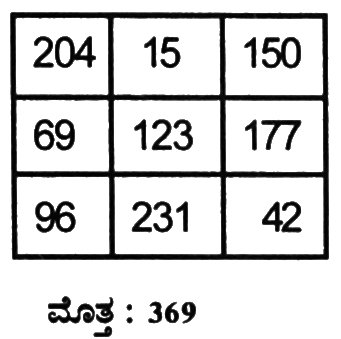
\includegraphics{src/figures/chap3/fig3-32.jpg}
\end{figure}

\begin{itemize}
	\item ಚಿತ್ರ  III.4. ಇದು 9 ಕ್ರಮವರ್ಗದ ಮಯಾಚೌಕ. ಹಾಗೂ 3 ಕ್ರಮವರ್ಗದ 9 ಮಾಯಾಚೌಕಗಳ ಗುಚ್ಛವೂ ಸಹ
	\item ಸೌಲಭ್ಯಕ್ಕಾಗಿ 1 ರಿಂದ 81 ಕ್ರಮಾಗತ ಸಂಖ್ಯೆಗಳನ್ನು ತೆಗೆದುಕೊಳ್ಳಲಾಗಿದೆ. ಯಾವುದೇ ಅಂಕಗಣಿತ ಶ್ರೇಢಿಯ 81 ಕ್ರಮಾಗತ ಸಂಖ್ಯೆಗಳನ್ನು ಬಳಸಿ ಈ ವಿಧಾನದಿಂದ 9 ಕ್ರಮವರ್ಗದ ಮಾಯಾಚೌಕ ರಚಿಸಬಹುದು.
	\item I.3ರಲ್ಲಿರುವ ವಿಧಾನದಿಂದ ರಚಿಸಿದರೆ ಬರುವ 9 ಕ್ರಮವರ್ಗದ ಮಾಯಾಚೌಕಕ್ಕೂ, ಇಲ್ಲಿ ರಚಿಸಿರುವ ಮಾಯಾಚೌಕಕ್ಕೂ ಇರುವ ವ್ಯತ್ಯಾಸಗಳನ್ನು ಗಮನಿಸಿ.
\end{itemize}
\begin{center}
$******$
\end{center}

12 ಕ್ರಮವರ್ಗದ ಮಾಯಾಚೌಕವನ್ನು ಗುಚ್ಛ ಮಾಯಾಚೌಕ ವಿಧಾನದಲ್ಲಿ ರಚಿಸಲು ಎರಡು ಭಿನ್ನ ಮಾರ್ಗಗಳಿವೆ. 3 ಕ್ರಮವರ್ಗದ 16 ಮಾಯಾಚೌಕಗಳನ್ನು ಗುಚ್ಛವಾಗಿಸುವುದು ಮತ್ತು 4 ಕ್ರಮವರ್ಗದ 9 ಮಾಯಾಚೌಕಗಳನ್ನುಗುಚ್ಛವಾಗಿಜೋಡಿಸುವುದು.ಇವೆರಡನ್ನೂ ಪರಿಶೀಲಿಸೋಣ.

ಮೊದಲನೆಯದಾಗಿ $4 \times 4$ರ 9 ಮಾಯಾಚೌಕಗಳನ್ನು ಬಳಸೋಣ. ಮೊತ್ತ 870
\begin{figure}[h]
\includegraphics{src/figures/chap3/fig3-33.eps}
\end{figure}

\begin{figure}[h]
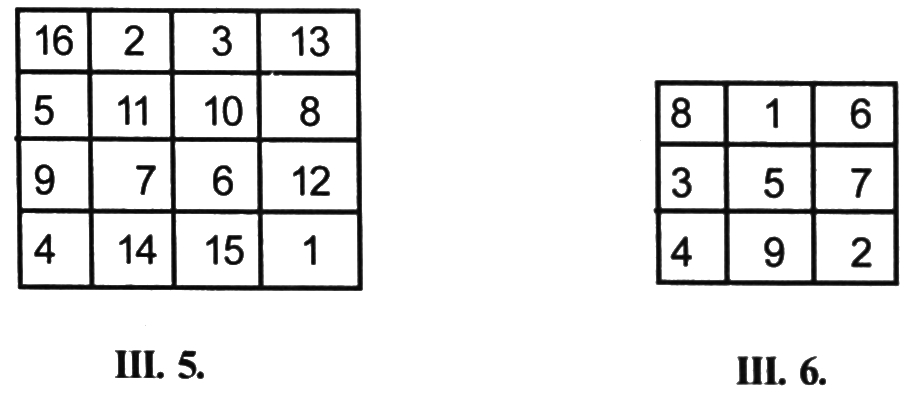
\includegraphics{src/figures/chap3/fig3-34.jpg}
\end{figure}

\begin{itemize}
	\item $12 \times 12$ರ ಚೌಕ ರಚಿಸಿ
	\item 9 ಸಮಭಾಗಗಳಾಗಿ ಅಂದರೆ $4 \times 4$ಚೌಕಗಳಾಗಿ ವಿಭಾಗಿಸಿ
	\item  III.6. ಚೌಕದಲ್ಲಿ 1 ಇರುವ ಸ್ಥಾನಕ್ಕೆ ಅನುರೂಪವಾಗಿ  III.7. ಚೌಕದಲ್ಲಿ ಬರುವ $4 \times 4$ (ಮೇಲಿನ ಅಡ್ಡಸಾಲಿನ ಮಧ್ಯದ $4 \times 4$ಚೌಕ) $4 \times 4$ ಚೌಕದಲ್ಲಿ 4 ಕ್ರಮವರ್ಗದ ಮಾಯಾಚೌಕ ರಚಿಸಿ. ಚಿತ್ರ  III.5 ರಂತೆ.
	\item  III.6.ಚೌಕದಲ್ಲಿ 2 ಇರುವ ಸ್ಥಾನಕ್ಕೆ ಅನುರೂಪವಾಗಿ  III.7. ಚೌಕದಲ್ಲಿ ಬರುವ $4 \times 4$ ಚೌಕದಲ್ಲಿ (ಕೆಳಅಡ್ಡಸಾಲಿನ ಕೊನೆಯ $4 \times 4$ ಚೌಕ) 4 ಕ್ರಮವರ್ಗದ ಮಾಯಾಚೌಕ 
	ರಚಿಸಿ. 17 ರಿಂದ 32 ಕ್ರಮಾಗತ ಸಂಖ್ಯೆ ಬಳಸಿ. ಹೀಗೆ ರಚಿಸಲು ಸುಲಭವಿಧಾನ ವೆಂದರೆ,  III.7.ರ ಮೇಲಿನ ಅಡ್ಡಸಾಲಿನ ಮಧ್ಯದ $4 \times 4$ ಚೌಕದಲ್ಲಿ ರಚಿಸಿರುವ ಮಾಯಾಚೌಕದ ಸಂಖ್ಯೆಗಳಿಗೆ 16ಸೇರಿಸಿ ಅನುರೂಪ ಮನೆಗಳಲ್ಲಿ ತುಂಬಿಸುವುದು.
	\item ಹೀಗೆಯೇ ಮೇಲಿನ ಹಂತದಲ್ಲಿ ರಚಿಸಿರುವ $4 \times 4$ ಮಾಯಾಚೌಕದ ಸಂಖ್ಯೆಗಳಿಗೆ 16ಸೇರಿಸಿ  III.6.ರಲ್ಲಿ 3 ಎಂದು ಬರೆದಿರುವ ಸ್ಥಾನದಲ್ಲಿರುವ (ಮೊದಲ ಕಂಭಸಾಲಿನ ಮಧ್ಯದ $4 \times 4$ ಚೌಕ) $4 \times 4$ ಚೌಕದಲ್ಲಿ ಅನುರೂಪ ಮನೆಗಳಿಗೆ ತುಂಬಿಸಿ. 33ರಿಂದ 48ವರೆಗೆ ಸಂಖ್ಯೆಗಳು ಬರುತ್ತವೆ.
	\item ಮುಂದೆ ಈ ಕೆಳಗಿನಂತೆ ಸಂಖ್ಯೆಗಳನ್ನು ತುಂಬಿಸಿ.

	49ರಿಂದ 64 ರವರೆಗಿನ ಸಂಖ್ಯೆಗಳನ್ನು  III.6.ರ 4 ಸ್ಥಾನಕ್ಕೆ ಅನುರೂಪ ಚೌಕದಲ್ಲಿ

	65ರಿಂದ 80 ರವರೆಗಿನ ಸಂಖ್ಯೆಗಳನ್ನು  III.6.ರ 5 ಸ್ಥಾನಕ್ಕೆ ಅನುರೂಪ ಚೌಕದಲ್ಲಿ

	81ರಿಂದ 96 ರವರೆಗಿನ ಸಂಖ್ಯೆಗಳನ್ನು  III.6.ರ 6 ಸ್ಥಾನಕ್ಕೆ ಅನುರೂಪ ಚೌಕದಲ್ಲಿ

	97ರಿಂದ 112 ರವರೆಗಿನ ಸಂಖ್ಯೆಗಳನ್ನು  III.6.ರ 7 ಸ್ಥಾನಕ್ಕೆ ಅನುರೂಪ ಚೌಕದಲ್ಲಿ

	113ರಿಂದ 128 ರವರೆಗಿನ ಸಂಖ್ಯೆಗಳನ್ನು  III.6.ರ 8 ಸ್ಥಾನಕ್ಕೆ ಅನುರೂಪ ಚೌಕದಲ್ಲಿ

	129ರಿಂದ 144 ರವರೆಗಿನ ಸಂಖ್ಯೆಗಳನ್ನು  III.6.ರ 9 ಸ್ಥಾನಕ್ಕೆ ಅನುರೂಪ ಚೌಕದಲ್ಲಿ ತುಂಬಿಸಿ.

	III.7.ರಲ್ಲಿ $4 \times 4$ ಚೌಕಗಳ 9 ಭಾಗಗಳೂ 4 ಕ್ರಮವರ್ಗದ ಮಾಯಾಚೌಕ ಗಳಾಗಿರುತ್ತವೆ.  III.7.ರಲ್ಲಿನ $12 \times 12$ ಚೌಕವು 12 ಕ್ರಮವರ್ಗದ ಮಾಯಾಚೌಕ. ಮೊತ್ತ 870

	9 ಭಾಗಗಳನ್ನು ಪ್ರತ್ಯೇಕವಾಗಿ ಗುರುತಿಸಲು ಅನುಕೂಲವಾಗುವಂತೆ ಕೆಲವು $4 \times 4$ಚೌಕಗಳನ್ನು ಮಸುಕು ಮಾಡಲಾಗಿದೆ.
\end{itemize}

\textbf{12 ಕ್ರಮವರ್ಗದ ಗುಚ್ಛ ಮಾಯಾಚೌಕ ರಚಿಸಲು 2ನೇ ವಿಧಾನ :}
\begin{itemize}
	\item $12 \times 12$ ಚೌಕ ರಚಿಸಿ. ಚಿತ್ರ  III.8
	\item ಇದನ್ನು 16 ಸಮಭಾಗಮಾಡಿ. ಪ್ರತಿಭಾಗವೂ $3 \times 3$ಚೌಕ ಆಗಿರುತ್ತದೆ. ನಾಲ್ಕು ಅಡ್ಡಸಾಲುಗಳಲ್ಲಿಯೂ ಮತ್ತು ನಾಲ್ಕು ಕಂಭಸಾಲುಗಳಲ್ಲಿಯೂ $3 \times 3$ಚೌಕಗಳಿರುತ್ತವೆ. ಒಟ್ಟಿನಲ್ಲಿ $3 \times 3$ ಇರುವ 16ಚೌಕಗಳ ಗುಚ್ಛ.
	\item ಸೌಲಭ್ಯಕ್ಕಾಗಿ 4 ಕ್ರಮವರ್ಗದ ಒಂದು ಮಾಯಾಚೌಕವನ್ನು ಬದಿಯಲ್ಲಿ ರಚಿಸಿ. ಸಂಖ್ಯೆಗಳು 1ರಿಂದ 16 ಇರಲಿ. ಚಿತ್ರ  III.9
	\item III.8. ಚೌಕ ($12 \times 12$)ದಲ್ಲಿ ಕೆಳತುದಿಯ ಬಲಗಡೆ ಮೂಲೆಯಲ್ಲಿರುವ $3 \times 3$ಚೌಕದಲ್ಲಿ 1ರಿಂದ 9 ವರೆಗಿನ ಸಂಖ್ಯೆಗಳನ್ನು ಬಳಸಿ ಮಾಯಾಚೌಕ ರಚಿಸಿ. (I.3 ವಿಧಾನ)
	\item ಇದು  III.8ರಲ್ಲಿನ 1 ರ ಸ್ಥಾನ ಎಂದು ಭಾವಿಸಿ.
	\item  III.9 ರಲ್ಲಿನ 2ಸ್ಥಾನಕ್ಕೆ ಅನುರೂಪವಾಗಿ, ಬರುವ  III.8 ರಲ್ಲಿನ $3 \times 3$ಚೌಕವನ್ನು 10ರಿಂದ 18ರವರೆಗಿನ ಸಂಖ್ಯೆ ಬಳಸಿ I.3 ವಿಧಾನದಿಂದ ಮಾಯಾಚೌಕ ರಚಿಸಿ.

	\item ಹೀಗೆಯೇ ಮುಂದುವರಿಸಿ  III.9ರಲ್ಲಿನ 3ರಿಂದ 16ವರೆಗಿನ ಸಂಖ್ಯೆಗಳಿಗೆ ಅನುರೂಪಸ್ಥಾನಗಳಲ್ಲಿ ಬರುವ  III.8ರ $3 \times 3$ಚೌಕಗಳಲ್ಲಿ 19ರಿಂದ 144ರವರೆಗಿನ ಸಂಖ್ಯೆಗಳನ್ನು ಪ್ರತಿ $3 \times 3$ ಚೌಕದಲ್ಲಿಯೂ 9 ಸಂಖ್ಯೆಗಳು ಕ್ರಮವಾಗಿ ಬರುವಂತೆ ತುಂಬಿಸಿ ಚಿತ್ರ. III.8ನೋಡಿ.
	\begin{figure}[h]
	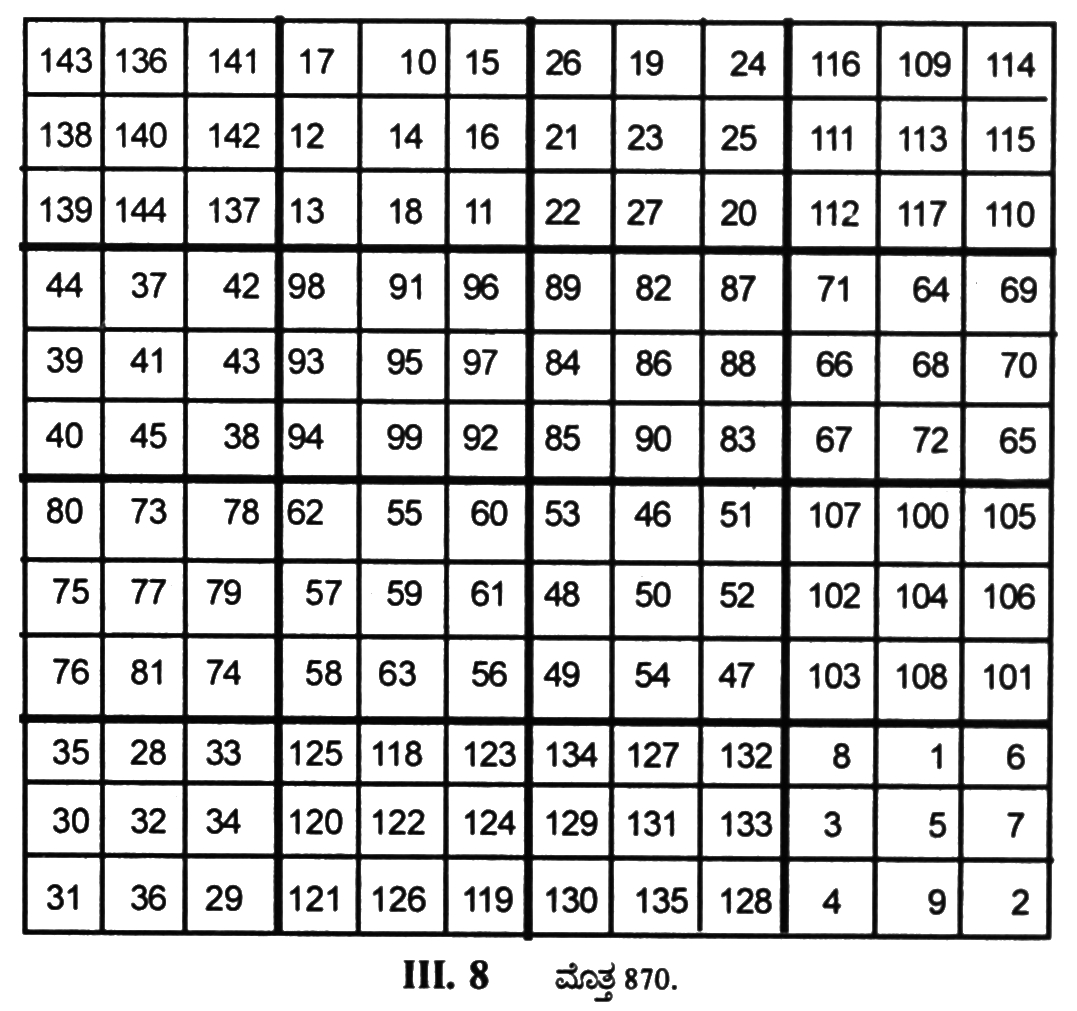
\includegraphics{src/figures/chap3/fig3-35.jpg}
	\end{figure}

	\begin{figure}[h]
	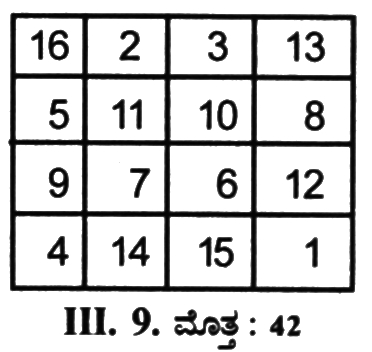
\includegraphics{src/figures/chap3/fig3-36.jpg}
	\end{figure}

	ಇದೇ ವಿಧಾನದಲ್ಲಿ 15 ಕ್ರಮವರ್ಗದ ಮಾಯಾಚೌಕವನ್ನು ರಚಿಸಿ ತೋರಿಸಲಾಗಿದೆ. $5 \times 5$ ಮನೆಗಳ 9 ಚೌಕಗಳ ಗುಚ್ಛ . ಮೊತ್ತ 1695
	\begin{figure}[H]
	\includegraphics{src/figures/chap3/fig3-37.eps}
	\end{figure}

	ಇದನ್ನೇ ಅಂದರೆ 15 ಕ್ರಮವರ್ಗದ ಮಾಯಾಚೌಕವನ್ನು $3 \times 3$ಮನೆಗಳುಳ್ಳ 25 ಚೌಕಗಳ ಗುಚ್ಛವಾಗಿಯೂ ರಚಿಸಬಹುದು. ಆಗ ಮಾಡಬೇಕಾದುದು ಇಷ್ಟೇ. 1ರಿಂದ 25 ವರೆಗಿನ ಕ್ರಮಾಗತ ಸಂಖ್ಯೆಗಳನ್ನು ಬಳಸಿ 5 ಕ್ರಮವರ್ಗದ ಮಾಯಾಚೌಕ ರಚಿಸಿ. $15 \times 15$ರ ಚೌಕವನ್ನು $3 \times 3$ರ ಚೌಕಗಳ 25 ಸಮಭಾಗಗಳಾಗಿ ವಿಭಾಗಿಸುವುದು. 5 ಕ್ರಮವರ್ಗದ ಮಾಯಾಚೌಕದಲ್ಲಿನ ಸಂಖ್ಯೆಗಳ (1ರಿಂದ 25) ಅನುರೂಪ ಸ್ಥಾನಗಳಲ್ಲಿ ಬರುವ $15 \times 15$ಚೌಕದಲ್ಲಿನ $3 \times 3$ಚೌಕಗಳಲ್ಲಿ 1 ರಿಂದ 9, 10ರಿಂದ 18, .....ಹೀಗೆ ಸಂಖ್ಯೆಗಳನ್ನು ತುಂಬಿಸಿ. 25 ಮಾಯಾಚೌಕ ರಚಿಸುವುದು. ಪ್ರಯತ್ನಿಸಿ. ಸಫಲರಾದರೆ, ಮೇಲಿನ  III.10. ಚೌಕಕ್ಕೂ ಅದಕ್ಕೂ ಇರುವ ವ್ಯತ್ಯಾಸಗಳನ್ನು ನೋಡಿ. ಗುಚ್ಛದ ಬೇರೆ ಬೇರೆ ಮಾಯಾಚೌಕಗಳನ್ನು ಗುರುತಿಸಲು ಅನುಕೂಲವಾಗುವಂತೆ.  III.10.ರಲ್ಲಿ ಕೆಲವನ್ನು ಮಸುಕು ಮಾಡಿದೆ.

	ಆಸಕ್ತರು ಇದೇ ವಿಧಾನ ಅನುಸರಿಸಿ ಬೇರೆಬೇರೆ ಕ್ರಮವರ್ಗಗಳ ಮಾಯಾಚೌಕ ರಚಿಸಿ ಆನಂದಿಸಬಹುದು.

	18 ಕ್ರಮವರ್ಗ - $6 \times 6$ರ 9 ಚೌಕ

	20 ಕ್ರಮವರ್ಗ - $4 \times 4$ರ 25 ಚೌಕಗಳು ಅಥವಾ $5 \times 5$ ರ 16 ಚೌಕಗಳು

	24 ಕ್ರಮವರ್ಗ - $6 \times 6$ರ 16 ಚೌಕಗಳು ಅಥವಾ $3 \times 3$ ರ 64 ಚೌಕಗಳು

	27 ಕ್ರಮವರ್ಗ - $9 \times 9$ರ 9 ಚೌಕಗಳು ಅಥವಾ $3 \times 3$ ರ 81 ಚೌಕಗಳು

	30 ಕ್ರಮವರ್ಗ - $6 \times 6$ರ 25 ಚೌಕಗಳು ಅಥವಾ $5 \times 5$ ರ 36 ಚೌಕಗಳು
\end{itemize}
\section*{IV. ಕೆಲವು ವಿಶಿಷ್ಟ ವಿಧಾನಗಳು :-}

ಮಾಯಾಚೌಕಗಳನ್ನು ರಚಿಸಲು ನಿರ್ದಿಷ್ಟ ವಿಧಾನಗಳನ್ನು ಹಿಂದಿನ ಅಧ್ಯಾಯಗಳಲ್ಲಿ ತಿಳಿಯಲಾಗಿದೆ. ಮತ್ತೂ ಹಲವಾರು ವಿಧಾನಗಳಲ್ಲಿ ಮಾಯಾಚೌಕ ರಚಿಸಲು ಸಾಧ್ಯ. ಆದರೆ ಈ ವಿಧಾನಗಳು ಎಲ್ಲ ಸಂದರ್ಭಗಳಿಗೂ ಅನ್ವಯಿಸದೇ ಕೆಲವು ವಿಶಿಷ್ಟ ಸಂದರ್ಭಗಳಿಗೆ ಮಾತ್ರ ಉಪಯೋಗವಾಗುತ್ತವೆ.

ಅಂತಹ ಕೆಲವನ್ನು ನೋಡೋಣ. IV. 1

\textbf{3. ಕ್ರಮವರ್ಗದ ಮಾಯಾಚೌಕ ರಚಿಸಲು ಶ್ಲೋಕ ರೂಪದ ಒಂದು ಸೂತ್ರ ಹೀಗಿದೆ.}

\begin{quote}
\textbf{ಶ್ಲೋಕ :}\\
\textbf{ಇಂದ್ರೋ ವಾಯುರ್ ಯಮಶ್ಬೈವ ನೈಋತ್ಯೋ ಮಧ್ಯಮ ಸ್ಥಿತಃ ।}\\
\textbf{ಈಶಾನಶ್ಚ ಕುಬೇರಶ್ಚ ಅಗ್ನಿರ್ ವರುಣ ಏವಚ ॥}
\end{quote}
ಎಂಟು ದಿಕ್ಕುಗಳಿಗೂ ಒಡೆಯರಾಗಿ ಅಷ್ಟದಿಕ್ಪಾಲಕರಿದ್ದಾರೆಂಬುದು ನಂಬಿಕೆ. ಇವುಗಳನ್ನು ಈ ಚಿತ್ರದಲ್ಲಿ ನಮೂದಿಸಿದೆ. ಹಾಗೆಯೇ ದಿನನಿತ್ಯದ ವ್ಯವಹಾರದಲ್ಲಿ ಬಳಸುವ ದಿಕ್ಕುಗಳ ಹೆಸರನ್ನೂ ಬರೆದಿದೆ.
\begin{itemize}
	\item $3 \times 3$ ರ ಚೌಕ ರಚಿಸಿದೆ
	\item 1 ರಿಂದ 9 ಸಂಖ್ಯೆ ತೆಗೆದುಕೊಂಡಿದೆ
	\item ಇಂದ್ರೋ - 1 ನ್ನು ಪೂರ್ವದ ಮನೆಯಲ್ಲಿ ತುಂಬಿದೆ
	\begin{figure}[h]
	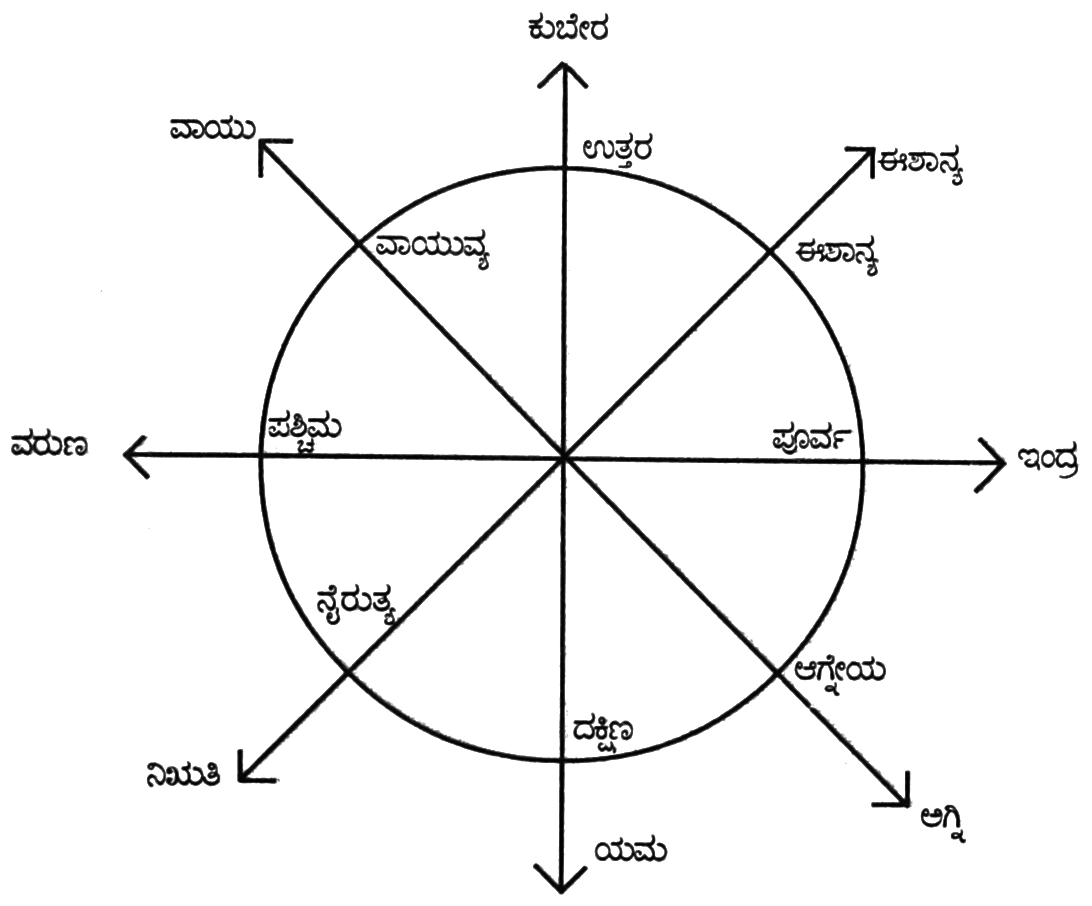
\includegraphics{src/figures/chap3/fig3-38.jpg}
	\end{figure}
	\begin{figure}[h]
	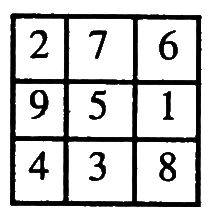
\includegraphics{src/figures/chap3/fig3-39.jpg}
	\end{figure}
	\item ವಾಯುರ್ - 2 ನ್ನು ವಾಯುವ್ಯದ ಮನೆಯಲ್ಲಿ ತುಂಬಿದೆ
	\item ಯಮ - 3 ನ್ನು ದಕ್ಷಿಣದ ಮನೆಯಲ್ಲಿ ತುಂಬಿದೆ
	\item ನೈಋತ್ಯೋ - 4 ನ್ನು ನೈಋತ್ಯದ ಮನೆಯಲ್ಲಿ ತುಂಬಿದೆ
	\item ಮಧ್ಯಮ - 5 ನ್ನು ಮಧ್ಯದ ಮನೆಯಲ್ಲಿ ತುಂಬಿದೆ
	\item ಉಳಿದ ಸಂಖ್ಯೆಗಳಾದ 6,7,8,9ಗಳನ್ನು ಕ್ರಮವಾಗಿ ಈಶಾನ್ಯ, ಉತ್ತರ (ಕುಬೇರ), ಆಗ್ನೇಯ, (ಅಗ್ನಿ), ಪಶ್ಚಿಮ (ವರುಣ)ದಿಕ್ಕಿನ ಮನೆಗಳಲ್ಲಿ ತುಂಬಿಸಿದೆ. ಮಾಯಾಚೌಕ ಸಿದ್ಧ. ಅಂಕಗಣಿತ ಶ್ರೇಢಿಯ ಯಾವುದೇ 9 ಸಂಖ್ಯೆಗಳನ್ನು ಬಳಸಬಹುದು.
\end{itemize}

\subsection*{IV. 2. ಅಪೇಕ್ಷಿತ ಸಮಸಂಖ್ಯೆ ಮೊತ್ತದ 4 ಕ್ರಮವರ್ಗದ ರಚನೆ :}

ಒಂದು ಸಮಸಂಖ್ಯೆಯಷ್ಟು ಮೊತ್ತ ಬರಬೇಕು, ಅದು 4 ಕ್ರಮವರ್ಗದ ಮಾಯಾಚೌಕವಾಗಿರಬೇಕು. ಇದನ್ನು ರಚಿಸಲು ಪ್ರಾಚೀನ ಭಾರತೀಯ ಗಣಿತಜ್ಞರು ಒಂದು ಸೂತ್ರವನ್ನು ಶ್ಲೋಕ ರೂಪದಲ್ಲಿ ಕೊಟ್ಟಿದ್ದಾರೆ.
\begin{quote}
\textbf{ಶ್ಲೋಕ :ವಾಂಛಾಕೃತಾರ್ಧಂ ಕೃತಮೇಕ ಹೀನಂ}\\
\textbf{ದ್ವ್ಯಂಕೇ ಗ್ರಹೇ ಷೋಡಶ ಸಪ್ತನಾಗೇ ।}\\
\textbf{ತಿಥೌ ದಿಶಾಯಾಂ ಪ್ರಥಮೇಚ ಕೋಷ್ಠೇ}\\
\textbf{ದ್ವಿ ಸಪ್ತ ಷಟ್ ತ್ರ್ಯಷ್ಟ ಕು ವೇದ ಬಾಣಾಃ ॥}
\end{quote}

ಇದನ್ನು ಅರ್ಥೈಸಿಕೊಳ್ಳಲು ಉದಾಹರಣೆಯಾಗಿ ಒಂದು ಮಾಯಾಚೌಕ ರಚಿಸೋಣ.
\begin{itemize}
	\item $4 \times 4$ರ ಎರಡು ಚೌಕ ರಚಿಸಿ.
	\item ಒಂದು ಚೌಕದಲ್ಲಿ 1 ರಿಂದ 16 ವರೆಗೆ ಕ್ರಮವಾಗಿ ಸಂಖ್ಯೆ ತುಂಬಿಸಿ. ಈ ಸಂಖ್ಯೆಗಳು ಅವಿರುವ ಮನೆಗಳ ಸ್ಥಾನ ಸೂಚಕಗಳು. ಚಿತ್ರ IV. 2.1. ನೋಡಿ,
	\begin{figure}[h]
	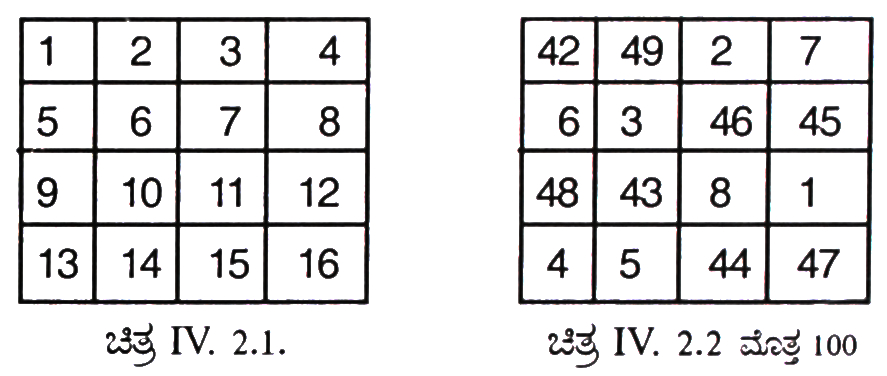
\includegraphics{src/figures/chap3/fig3-40.jpg}
	\end{figure}
	\item ಅಪೇಕ್ಷಿತ ಮೊತ್ತ 100 ಇರಲಿ.
	\item \textbf{‘ವಾಂಛಾಕೃತಾರ್ಧಂ’ - ‘ಅಪೇಕ್ಷಿತ’} ಮೊತ್ತದ ಅರ್ಧ ತೆಗೆದುಕೊಳ್ಳಿ - 50
	\item \textbf{‘ಕೃತ ಮೇಕ ಹೀನಂ’-} ಒಂದೊಂದನ್ನೇ ಕಳೆಯಿರಿ. ಎಂಟು ಸಂಖ್ಯೆ ತೆಗೆದುಕೊಳ್ಳಿ. - 49,48,47,46,45,44,43,42
	\item ಈ ಸಂಖ್ಯೆಗಳನ್ನು ಶ್ಲೋಕದ 2 ಮತ್ತು 3ನೇ ಪಾದಗಳು ಹೇಳುವಂತೆ ತುಂಬಿಸಿ.

	\textbf{ದ್ವ್ಯಂಕೇ - }ಎರಡನೇ ಮನೆ - 49;

	\textbf{ಗ್ರಹೇ -} ನವಗ್ರಹಗಳು - 9ನೇ ಮನೆ -48;

	\textbf{ಷೋಡಶ -} 16ನೇ ಮನೆ - 47;

	\textbf{ಸಪ್ತ -} ಏಳನೇ ಮನೆ - 46;

	\textbf{ನಾಗೇ -} ಅಷ್ಟದಿಗ್ಗಜಗಳು - 8ನೇ ಮನೆ -45;

	\textbf{ತಿಥೌ -} ತಿಥಿಗಳು 15 - 15ನೇ ಮನೆ -44;

	\textbf{ದಿಶಾಯಾಂ -} ದಶದಿಕ್ಕುಗಳು - 10ನೇ ಮನೆ -43;

	\textbf{ಪ್ರಥಮೇ -} 1ನೇ ಮನೆ - 42

	\item ಉಳಿದ ಖಾಲಿ ಮನೆಗಳನ್ನು ಶ್ಲೋಕದ ಕೊನೆಯ ಪಾದದ ಅನುಸಾರವಾಗಿ ಅವು ಸೂಚಿಸುವ ಸಂಖ್ಯೆಗಳಿಂದ ಕ್ರಮವಾಗಿ ತುಂಬಿಸಿ.

	ದ್ವಿ  - 2, ಸಪ್ತ -7, ಷಟ್-6,  ತ್ರಿ 3, ಅಷ್ಟ -8, ಕು -1, ವೇದ -4, ಬಾಣಾಃ-5, ಮಾಯಾಚೌಕ ಲಭ್ಯ. ಮೊತ್ತ 100 ಚಿತ್ರ IV.2.2.ನೋಡಿ.
	\begin{center}
	****
	\end{center}
\end{itemize}

\subsection*{IV. 3-. 5. ಕ್ರಮವರ್ಗದ ಅಪೇಕ್ಷಿತ ಮೊತ್ತದ ಮಾಯಾಚೌಕ ರಚನೆ :}

ನಮಗೆ ಇಷ್ಟ ಬಂದಷ್ಟು ಮೊತ್ತವಿರುವಂತೆ 5 ಕ್ರಮವರ್ಗದ ಮಾಯಾಚೌಕ ರಚಿಸಲು ಸಿದ್ಧ ವಿಧಾನವಿದೆ. ಅಷ್ಟಾವಧಾನ ಕಾರ್ಯಕ್ರಮದ ಗಣಿತಾವಧಾನದಲ್ಲಿ ಅವಧಾನಿಗಳು ಈ ವಿಧಾನ ಅನುಸರಿಸುತ್ತಾರೆ.
\begin{itemize}
	\item ಇದರಲ್ಲಿ ಒಂದು ಆಧಾರ ಚೌಕವಿರುತ್ತದೆ. ಮೊತ್ತ ಎಷ್ಟಾದರೂ ಈ ಚೌಕ ಬದಲಾಗುವುದಿಲ್ಲ. ಚಿತ್ರ IV. 3.1
	\item ಇದರಲ್ಲಿ ಧನ ಮತ್ತು ಋಣ ಪೂರ್ಣಾಂಕಗಳು ಇವೆ.
	\item ಕೇಂದ್ರ ಮನೆ ಖಾಲಿ ಇದೆ.
	\item ಪ್ರತಿ ಅಡ್ಡಸಾಲು, ಕಂಭಸಾಲು ಮತ್ತು ಕರ್ಣಗಳಲ್ಲಿನ ಸಂಖ್ಯೆಗಳ ಮೊತ್ತ 0.

	ಉದಾಹರಣೆ : ಅಪೇಕ್ಷಿತ ಮೊತ್ತ 300 ಇರಲಿ
	\begin{figure}[h]
	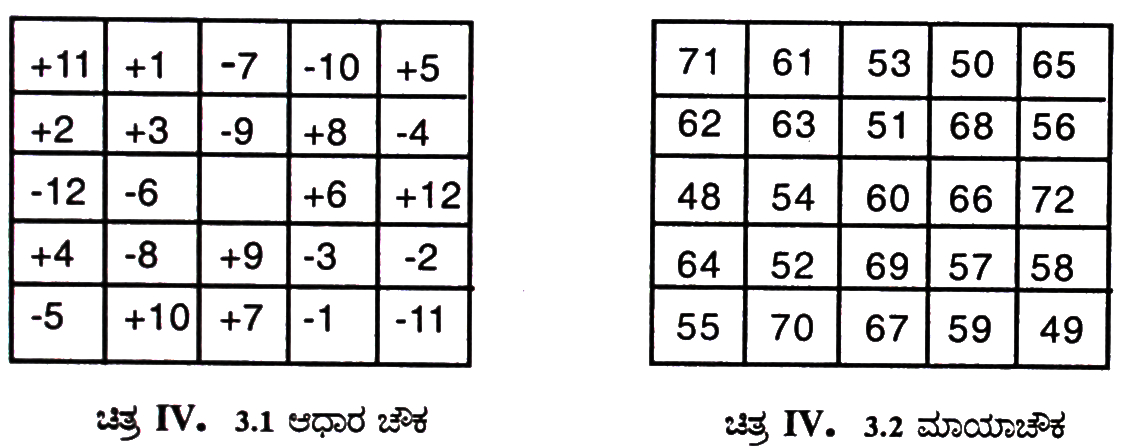
\includegraphics{src/figures/chap3/fig3-41.jpg}
	\end{figure}
	\item ಇದನ್ನು 5 ರಿಂದ ಭಾಗಿಸಿ - $\frac{300}{5}=60$
	\item $5 \times 5$ಚೌಕವನ್ನು ರಚಿಸಿ (ಚಿತ್ರ IV.3.2) ಅದರ ಕೇಂದ್ರ ಮನೆಯಲ್ಲಿ 60ನ್ನು ತುಂಬಿಸಿ.
	\item ಉಳಿದ ಮನೆಗಳನ್ನು ಆಧಾರ ಚೌಕದಲ್ಲಿರುವ ಸಂಖ್ಯೆಗಳನ್ನು 60ಕ್ಕೆ ಕೂಡಿಸಿ/ಕಳೆದು ಅನುರೂಪಮನೆಗಳಲ್ಲಿ ತುಂಬಿಸಿ. ಮಾಯಾಚೌಕ ಲಭ್ಯ.ಚಿತ್ರ IV. 3.2
	\item ಅಪೇಕ್ಷಿತ ಮೊತ್ತವು 5ರಿಂದ ನಿಶ್ಶೇಷವಾಗಿ ಭಾಗವಾಗದೆ, ಶೇಷ ಉಳಿದರೆ ಈ ಕೆಳಗಿನ ವಿಧಾನ ಉಪಯೋಗಿಸಿ.

	\textbf{ಉದಾ :} ಅಪೇಕ್ಷಿತ ಮೊತ್ತ 303
	\item 5 ರಿಂದ ಭಾಗಿಸಿದಾಗ $\frac{303}{5}=60$ ಶೇಷ 3
	\item ಅಪೇಕ್ಷಿತ ಮೊತ್ತ 300 ಇರುವಂತೆ 5 ಕ್ರಮವರ್ಗದ ಮಾಯಾಚೌಕವನ್ನು ಮೇಲಿನ ವಿಧಾನದಿಂದ ರಚಿಸಿ.
	\item ಚಿತ್ರ IV. 3.3 ರಲ್ಲಿ ವೃತ್ತ ಹಾಕಿರುವ ಮನೆಗಳಲ್ಲಿ ಬರುವ ಸಂಖ್ಯೆಗಳಿಗೆ 3 (ಶೇಷ)ನ್ನು ಸೇರಿಸಿ ಬರೆಯಿರಿ. 303 ಮೊತ್ತದ ಮಾಯಾಚೌಕ ಲಭ್ಯ. ಚಿತ್ರ IV.3.4
	\begin{figure}[h]
	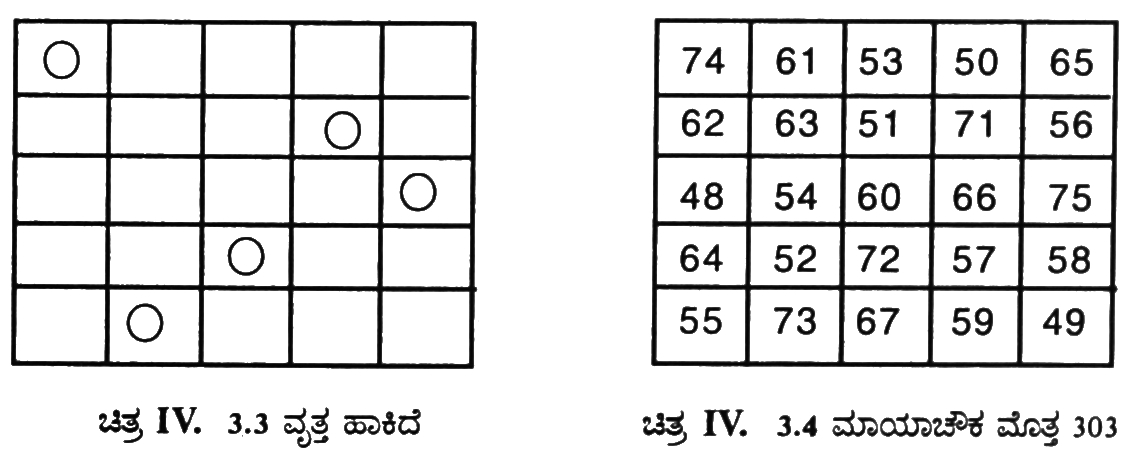
\includegraphics{src/figures/chap3/fig3-42.jpg}
	\end{figure}
\end{itemize}

\subsection*{IV. 4 ಕ್ಲಾಡ್ ಗಾಸ್ಪರ್ ಬಾಷೆಟ್ ವಿಧಾನ:}

\textbf{ಕ್ಲಾಡ್ ಗಾಸ್ಪರ್ ಬಾಷೆಟ್} (1581-1638) ಒಬ್ಬ ಜೆಸ್ಯೂಟ್ ಪಾದ್ರಿ. ಒಂದು ವರ್ಷ ಧರ್ಮಪ್ರಚಾರದಲ್ಲಿದ್ದ. ನಂತರ ಅನಾರೋಗ್ಯದ ಕಾರಣ ಆ ಕೆಲಸ ಬಿಟ್ಟ. ಉಳಿದ ಜೀವಮಾನವನ್ನೆಲ್ಲ ಫ್ರಾನ್ಸಿನಲ್ಲಿದ್ದ ತನ್ನ ಜಮೀನಿನಲ್ಲಿ ಇದ್ದುಕೊಂಡು, ಬಿಡುವಿನ ವೇಳೆ ಗಣಿತ ಸಮಸ್ಯೆಗಳ ಬಗ್ಗೆ ಪುಸ್ತಕಗಳನ್ನು ಬರೆದ. ಇವುಗಳ ಆಧಾರದ ಮೇಲೆ ಅನೇಕ ಗಣಿತೀಯ ಮನರಂಜನೆ ಗ್ರಂಥಗಳು ಹೊರಬಂದವು.

5 ಕ್ರಮವರ್ಗದ ಮಾಯಾಚೌಕ ರಚನೆಗೆ ಇವನು ಒಂದು ವಿಧಾನವನ್ನು ಸೂಚಿಸಿದ್ದಾನೆ. ಡಿ. ಲಾ ಲೌಬೆರೆ ವಿಧಾನಕ್ಕಿಂತ ಸ್ವಲ್ಪ ಭಿನ್ನವಾಗಿದೆ.

ಈ ವಿಧಾನ ಹೀಗಿದೆ :-
\begin{figure}[h]
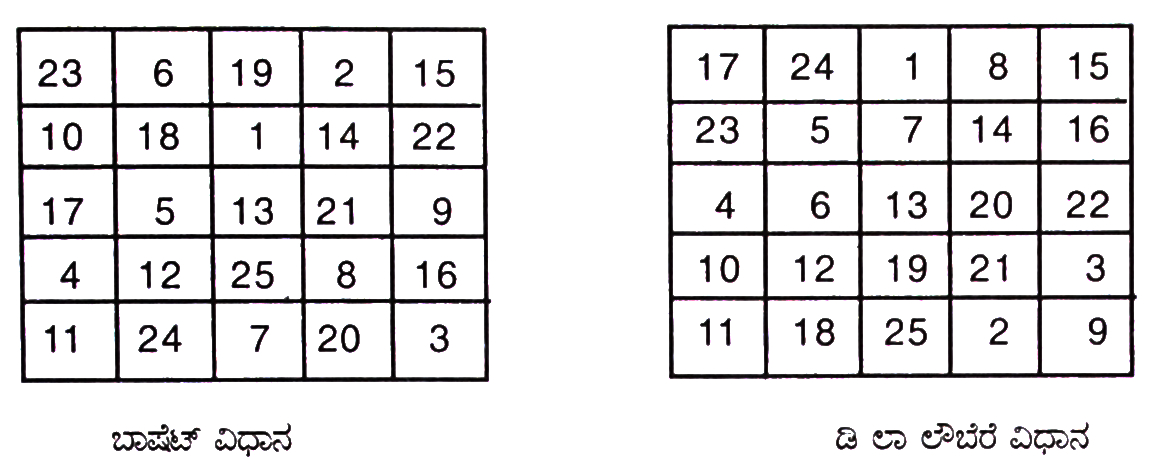
\includegraphics{src/figures/chap3/fig3-43.jpg}
\end{figure}

\begin{itemize}
	\item $5 \times 5$ಚೌಕದ ಕೇಂದ್ರ ಮನೆಯ ಮೇಲಿನ ಮನೆಯಿಂದ ಪ್ರಾರಂಭಿಸಿ. ಬಲಕ್ಕೆ ಓರೆಯಾಗಿ ಲೌಬೆರೆ ವಿಧಾನದಿಂದ ತುಂಬಿಸಿ.
	\item ತುಂಬಿದ ಮನೆ ಎದುರಾದಾಗ (ಇಲ್ಲಿ 5) ಎರಡು ಮನೆ ಮೇಲಕ್ಕೆ ಜಿಗಿದು ಸಂಖ್ಯೆಗಳನ್ನು ತುಂಬಿಸಿ.
	\item ಮೇಲಕ್ಕೆ ಮನೆಗಳಿಲ್ಲದಾಗ (10ರಲ್ಲಿ ಆಗುವಂತೆ) ಅದೇ ಸಾಲಿನ ಕೆಳ ತುದಿಯ ಖಾಲಿ ಮನೆ ತುಂಬಿಸಿ.
	\item ಬಲ ತುದಿಯ ಕಂಭಸಾಲಿನ ಮೇಲಿನ ಮನೆಗೆ ಬಂದಾಗ, ಅದೇ ಸಾಲಿನಲ್ಲಿ ಕೆಳಗೆ ಖಾಲಿ ಇರುವ ಮನೆ ತುಂಬಿಸಿ.
	\item ಹೋಲಿಕೆಗಾಗಿ ಲೌಬೆರೆ ಚೌಕವನ್ನು ಕೊಟ್ಟಿದೆ.
	\item ಬಾಷೆಟ್ ವಿಧಾನ ಕೇವಲ ಕುತೂಹಲ ಕಾರಕ.
\end{itemize}

\subsection*{IV. 5. ದಿನಾಂಕ ಮಾಯಾಚೌಕ :}

ಇಪ್ಪತ್ತನೆಯ ಶತಮಾನದಲ್ಲಿ ಜಗತ್ತು ಕಂಡ ಅತಿ ಪ್ರತಿಭಾವಂತ ಗಣಿತಜ್ಞ ಭಾರತೀಯ ಶ್ರೀನಿವಾಸ ರಾಮಾನುಜಂ ಅವರು. ಗಣಿತ ಕ್ಷೇತ್ರದಲ್ಲಿ ಅವರ ಸಾಧನೆ ಅದ್ಭುತ. ಅವರು ಮಾಯಾಚೌಕಗಳಲ್ಲೂ ಕೈಯಾಡಿಸಿದವರು. ವಿಶಿಷ್ಟ ವಿಧಾನ ರೂಪಿಸಿ ಮಾಯಾಚೌಕ ರಚಿಸಿದವರು. ಅವರು 4 ಕ್ರಮವರ್ಗದ ಮಾಯಾಚೌಕ ರಚಿಸಲು ಒಂದು ವಿಧಾನವನ್ನು ರೂಪಿಸಿದ್ದಾರೆ. ಆ ವಿಧಾನವನ್ನು ತಿಳಿಯೋಣ.

$A, B, C, D, P, Q, R, S$ ಪೂಣಾಂಕಗಳಾಗಿರಲಿ. ಇವುಗಳನ್ನು ಜೋಡಿಯಾಗಿ ತೆಗೆದುಕೊಂಡು ಮೊತ್ತ ಬರೆದರೆ $A+P, D+S.....$ ಇತ್ಯಾದಿ ಬರುತ್ತವೆ. ಈ ಜೋಡಿಗಳನ್ನು ಕೆಳಗೆ ಕೊಟ್ಟಿರುವಂತೆ $4 \times 4$ರ ಚೌಕದಲ್ಲಿ ಅಳವಡಿಸಿದರೆ ಮಾಯಾಚೌಕ ಲಭಿಸುತ್ತದೆ.

\begin{figure}[h]
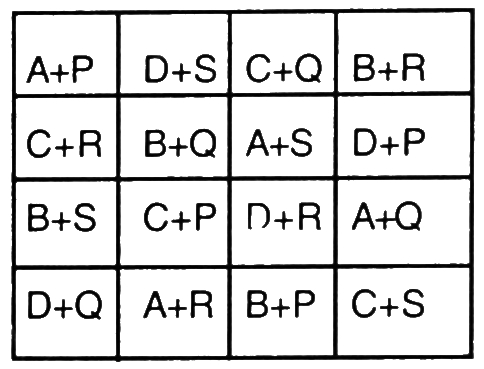
\includegraphics{src/figures/chap3/fig3-44.jpg}
\end{figure}

ಪ್ರತಿ ಅಡ್ಡಸಾಲು, ಕಂಭಸಾಲು ಮತ್ತು ಕರ್ಣಗಳ ಮನೆಗಳ ಸಂಖ್ಯೆಗಳ ಮೊತ್ತ. $A+B+C+ D+ P+ Q+ R+ S$ ಇರುವುದನ್ನು ಗಮನಿಸಿ.

ಈ ಜೋಡಣೆಯನ್ನು ಬಳಸಿ ಶ್ರೀನಿವಾಸರಾಮಾನುಜಂರವರ ಜನ್ಮ ಶತಾಬ್ದಿ ದಿನಾಂಕದ ಮಾಯಾಚೌಕ ರಚಿಸೋಣ.

ಜನ್ಮ ಶತಾಬ್ದಿ ದಿನಾಂಕ : 22-12-1987

ಇದನ್ನು 4 ಸಂಖ್ಯೆಗಳಾಗಿ ಬರೆದರೆ 22;12;19;87 ಬರುತ್ತವೆ.

\begin{tabular}{cccc}
A+P=22 & A=20; & P=2 & ಇರಲಿ\\
D+S=12 & D=1; & S=11 & ಇರಲಿ\\
C+Q=19 & C=13; & R=6 & ಇರಲಿ\\
B+R=87 & B=60; & R=27 & ಇರಲಿ
\end{tabular}

$4 \times 4$ ಚೌಕದಲ್ಲಿ ಇವುಗಳನ್ನು ಆದೇಶಿಸಿದರೆ ಕೆಳಗೆ ಕಾಣಿಸಿರುವ ಚೌಕಗಳು ದೊರೆಯುತ್ತವೆ.
\begin{figure}[h]
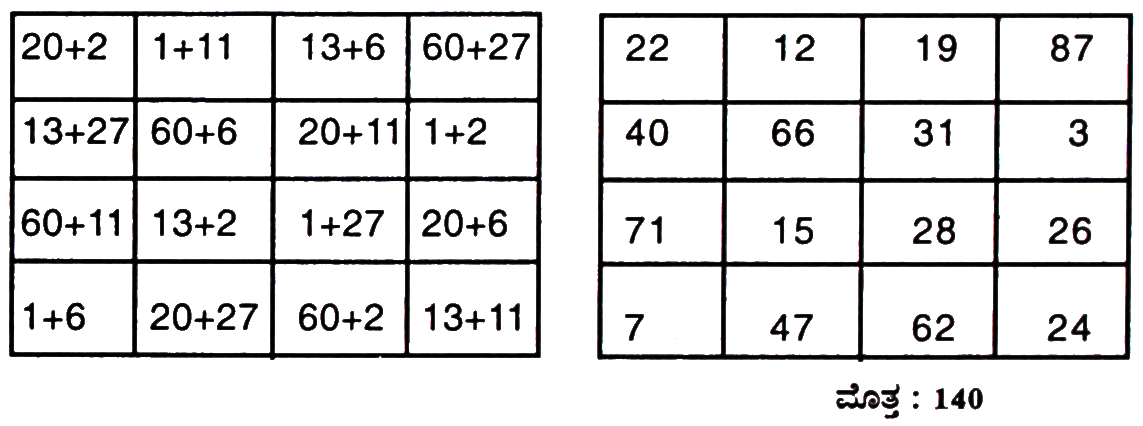
\includegraphics{src/figures/chap3/fig3-45.jpg}
\end{figure}

ಇದೇ ವಿಧಾನದಲ್ಲಿ ಯಾವುದೇ ದಿನಾಂಕದ ಮಾಯಾಚೌಕ ರಚಿಸಬಹುದು. ಸಂಖ್ಯೆಗಳು ಪುನರಾವರ್ತಿತವಾದರೆ, A+P ಇತ್ಯಾದಿಗಳ ಹಂಚಿಕೆ ಬದಲಿಸಿ ನಿವಾರಿಸಬಹುದು.

\textbf{ದಿನಾಂಕ ಮಾಯಾಚೌಕ ಮತ್ತೊಂದು ವಿಧಾನ :}

ದಿನಾಂಕವನ್ನು ಹೊಂದಿರುವ 4 ಕ್ರಮವರ್ಗದ ಮಾಯಾಚೌಕವನ್ನು ಇನ್ನೊಂದು ವಿಧಾನದಲ್ಲಿಯೂ ರಚಿಸಬಹುದು.

ಉದಾಹರಣೆಗೆ 15-8-2007ತೆಗೆದುಕೊಳ್ಳೋಣ.
\begin{itemize}
	\item $4 \times 4$ಚೌಕ ರಚಿಸಿ
	\begin{figure}[h]
	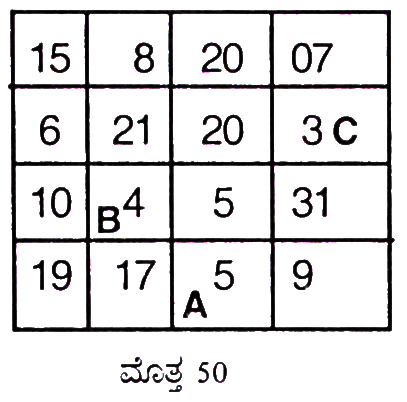
\includegraphics{src/figures/chap3/fig3-46.jpg}
	\end{figure}
	\item ಎರಡನೇ ಅಡ್ಡಸಾಲಿನ ಕೊನೆ ಮನೆ, 3ನೇ ಅಡ್ಡಸಾಲಿನ ಎರಡನೇ ಮನೆ 4ನೇ ಅಡ್ಡಸಾಲಿನ 3ನೆ ಮನೆಗಳಲ್ಲಿ ಯಾವುದಾದರೂ ಮೂರು ಧನ ಪೂರ್ಣಾಂಕಗಳನ್ನು ತುಂಬಿಸಿ. ಇವುಗಳನ್ನು $A,B,C$ ಅಕ್ಷರಗಳಿಂದ ಸೂಚಿಸಿದೆ. ಉದಾಹರಣೆಯಲ್ಲಿ 5,4,3 ತುಂಬಿಸಿದೆ.
	\item ಮೊದಲ ಅಡ್ಡಸಾಲಿನಲ್ಲಿ ಕೊಟ್ಟಿರುವ ದಿನಾಂಕ ತುಂಬಿಸಿ. ವರ್ಷ ಸೂಚಕವನ್ನು ಎರಡು ಸಮಭಾಗಮಾಡಿ. (15,8,20,07)
	\item 4 ಕ್ರಮವರ್ಗದ ವಿಶಿಷ್ಟ ಮಾಯಾಚೌಕವನ್ನು $2 \times 2$ಅಳತೆಯ 4ಸಮ ಭಾಗಗಳಾಗಿ ಮಾಡಿದಾಗ, ಆ 4 ಸಂಖ್ಯೆಗಳ ಮೊತ್ತವು ಮಾಯಾಚೌಕದ ಮೊತ್ತಕ್ಕೆ ಸಮವಾಗಿರುತ್ತದೆ. ಇಲ್ಲಿ ಮೊದಲ ಅಡ್ಡಸಾಲಿನ ಸಂಖ್ಯೆಗಳ ಮೊತ್ತ 50. ಹಾಗಾಗಿ ಬಲ ಮೇಲ್ಭಾಗದ $2 \times 2$ ಚೌಕದ ಮೊತ್ತ 50 ಇರಬೇಕು. ಅದರ ಮೂರು ಸಂಖ್ಯೆಗಳು 20,07,3 ತಿಳಿದಿವೆ. ಆದ್ದರಿಂದ ಉಳಿದ ಸಂಖ್ಯೆ 50 -(20+7+3) = 20 ಇರಬೇಕು ತುಂಬಿಸಿ.
	\item ಬಲ ಮೇಲ್ತುದಿಯಿಂದ ಎಡ ಕೆಳತುದಿಗೆ ಬರುವ ಕರ್ಣದ ಮೂರು ಸಂಖ್ಯೆಗಳು ತಿಳಿದಂತಾಗಿದೆ. 07,20,4. ಇವುಗಳ ಮೊತ್ತ 31 ಆದ್ದರಿಂದ ಖಾಲಿ ಇರುವ ಮನೆಯಲ್ಲಿ 50-31=19-ಇರಬೇಕು ತುಂಬಿಸಿ.
	\item ಮೂರನೆ ಕಂಭ ಸಾಲಿನಲ್ಲಿ 20,20,5ಇವೆ. ಹಾಗಾಗಿ ಖಾಲಿ ಇರುವ ಮನೆಯಲ್ಲಿ 50 -(20+20+5) = 5ಇರಬೇಕು. ತುಂಬಿಸಿ.
	\item ಮಧ್ಯದ ನಾಲ್ಕು ಮನೆಗಳ ಸಂಖ್ಯೆಗಳ ಮೊತ್ತ 50 ಬರಬೇಕು. ಬಂದಿರುವ ಸಂಖ್ಯೆಗಳು 20,4,5 ಆದ್ದರಿಂದ ಖಾಲಿ ಇರುವ ಮನೆಯಲ್ಲಿ 50 -(20+4+5) =21ಇರಬೇಕು ತುಂಬಿಸಿ.
	\item ಇನ್ನೊಂದು ಕರ್ಣದಲ್ಲಿ 15,21,5 ಇವೆ. ನಾಲ್ಕನೆಮನೆಯಲ್ಲಿ 50-(15+21+5) =9 ಇರಬೇಕು ತುಂಬಿಸಿ.
	\item ಮೇಲಿನ ಎಡಗಡೆಯ $2 \times 2$ಚೌಕ ಮತ್ತು ಬಲಗಡೆಯ ಕೆಳಗಿನ $2 \times 2$ಚೌಕಗಳಲ್ಲಿ ಪ್ರತಿಯೊಂದರಲ್ಲಿಯೂ 3 ಸಂಖ್ಯೆಗಳಿವೆ. ಇವುಗಳ ಮೊತ್ತ ಕಂಡುಹಿಡಿದು 50ಕ್ಕೆ ಪೂರಕವಾಗುವಂತೆ 4ನೆ ಸಂಖ್ಯೆ ತುಂಬಿಸಿ.
	\item ಉಳಿದ ಖಾಲಿ ಮನೆಗಳನ್ನು 50ರ ಪೂರಕ ಸಂಖ್ಯೆಯಿಂದ ತುಂಬಿಸಿ.
\end{itemize}

